\documentclass[english,oneside,a4paper,censored,csm,software-track-2020]{HYthesisML}

\usepackage{csquotes}

\usepackage[style=numeric,bibstyle=numeric,backend=biber,natbib=true,
            sorting=none,sortcites=true,maxbibnames=99,giveninits=true,uniquename=init]{biblatex}
\addbibresource{bibliography.bib}
\DeclareNameAlias{sortname}{family-given}
\defbibheading{bibliography}[\bibname]{%
  \chapter*{#1}%
  \markboth{#1}{#1}}

\usepackage[pdftex, plainpages=false]{hyperref} % For hyperlinks and pdf metadata
\usepackage{fancyhdr} 
\usepackage{array} % Ragged-right p-columns in the host table
\usepackage{longtable}
\usepackage{float} % [H] pins the key-terms glossary at the appendix heading
\usetikzlibrary{arrows.meta, positioning, automata, shapes.geometric, calc, fit, backgrounds}
\usepackage[section]{placeins} % flush pending floats before each \section
\renewcommand{\topfraction}{0.9}
\renewcommand{\textfraction}{0.08}
\renewcommand{\floatpagefraction}{0.75}

% Ragged-right paragraph column: avoids stretched inter-word spacing in narrow cells.
\newcolumntype{R}[1]{>{\raggedright\arraybackslash}p{#1}}

\onehalfspacing 

\sloppy
% Sentence-ending punctuation keeps the same interword space as the
% rest of the line. TeX's default extra glue after `.` is the gap
% after "gap." in the research-gap paragraph. Attached to babel's
% English extras so a language switch cannot put the extra glue back.
\addto\extrasenglish{\frenchspacing}
\AtBeginDocument{\frenchspacing}

% Median above a bootstrap interval, used by figures/tab_latency.tex.
\newcommand{\mci}[3]{%
  \begin{tabular}[t]{@{}r@{}}%
    $#1$\\[-2pt]{\scriptsize$[#2,\,#3]$}%
  \end{tabular}}

\title{Performance, Safety, and Engineering Trade-offs of Rust and C++ in Nokia RAN Control-Plane Systems}
\author{Ha Vien}
\date{11 September 2026}
\supervisors{Prof. Keijo Heljanko, Christoph Luneburg, Petteri Kotimaa}
\examiners{Prof. Keijo Heljanko}
\keywords{Rust, C++, RAN control plane, tail latency, memory safety, fault injection, incremental adoption}
\additionalinformation{\translate{\track}}


\classification{\protect{\ \\
\  Software and its engineering $\rightarrow$ Software notations and tools $\rightarrow$ General programming languages\  \\
\  Computer systems organization $\rightarrow$ Real-time systems $\rightarrow$ Real-time system specification\\
\  Networks $\rightarrow$ Network types $\rightarrow$ Mobile networks
}}

\hypersetup{
    %bookmarks=true,         % show bookmarks bar first?
    unicode=true,           % to show non-Latin characters in Acrobat’s bookmarks
    pdftoolbar=true,        % show Acrobat’s toolbar?
    pdfmenubar=true,        % show Acrobat’s menu?
    pdffitwindow=false,     % window fit to page when opened
    pdfstartview={FitH},    % fits the width of the page to the window
    pdftitle={Performance, Safety, and Engineering Trade-offs of Rust and C++ in Nokia RAN Control-Plane Systems},
    pdfauthor={Ha Vien},
    pdfsubject={Master's thesis, Computer Science},
    pdfcreator={Ha Vien},
    pdfproducer={pdfLaTeX}, % producer of the document
    pdfkeywords={Rust} {C++} {RAN control plane} {tail latency} {memory safety},
    pdfnewwindow=true,      % links in new window
    colorlinks=true,        % false: boxed links; true: colored links
    linkcolor=black,        % color of internal links
    citecolor=black,        % color of links to bibliography
    filecolor=magenta,      % color of file links
    urlcolor=cyan           % color of external links
}


% Generated by bench/plot_figures.py -- do not edit by hand.
\newcommand{\ReprLoad}{28}
\newcommand{\ReprLoadAch}{28.0}
\newcommand{\ReprLoadShortfall}{0.1}
\newcommand{\SatKnee}{334}
\newcommand{\TrackingLoad}{336}
\newcommand{\NRepeats}{20}
\newcommand{\NLoadLevels}{14}
\newcommand{\NVariants}{4}
\newcommand{\NRuns}{1120}
\newcommand{\PNineNineSpread}{14}
\newcommand{\PFiftySpread}{2.9}
\newcommand{\PFiftyRange}{3}
\newcommand{\PNineNineRange}{460}
\newcommand{\PNineNineMaxCI}{2540}
\newcommand{\MaxOfferedLoad}{784}
\newcommand{\NTests}{10}
\newcommand{\MinAttainableP}{0.0000019}
\newcommand{\CorrectedFloor}{0.000019}
\newcommand{\NSignificant}{2}
\newcommand{\SmallestHolm}{0.00010}
\newcommand{\NExclZero}{4}
\newcommand{\NTailExclZero}{1}
\newcommand{\TailExclZeroRows}{p99 latency under system}
\newcommand{\RobustExclZeroRows}{p50 latency, Peak RSS and CPU utilisation under system}
\newcommand{\PFiftyDiffAbsMax}{1.6}
\newcommand{\PFiftyDiffCIMax}{3}
\newcommand{\RssLangDiffLo}{1.3}
\newcommand{\RssLangDiffHi}{1.7}
\newcommand{\RssLangCILo}{-0.5}
\newcommand{\RssLangCIHi}{1.9}
\newcommand{\CpuDiffAbsMax}{3.4}
\newcommand{\CrossAllocConsistent}{p50 latency, p99 latency, p99.9 latency, Peak RSS and CPU utilisation}
\newcommand{\CrossAllocReversed}{none}
\newcommand{\NCrossAllocReversed}{0}
\newcommand{\RssAllocDiffLo}{55.9}
\newcommand{\RssAllocDiffHi}{56.5}
\newcommand{\BudgetRepeats}{15}
\newcommand{\BudgetCoreCpp}{34.4}
\newcommand{\BudgetCoreRust}{21.3}
\newcommand{\BudgetSvcCpp}{13.52}
\newcommand{\BudgetSvcRust}{12.63}
\newcommand{\BudgetHandoffCpp}{13.49}
\newcommand{\BudgetHandoffRust}{12.61}
\newcommand{\BudgetCoreShareMax}{0.250}
\newcommand{\BudgetCoreFaster}{Rust}
\newcommand{\BudgetCoreRatio}{1.6}
\newcommand{\BudgetHandoffSlower}{C++}
\newcommand{\BudgetBoundVsCore}{101}
\newcommand{\FfiCrossing}{2.54}
\newcommand{\FfiOpRepeats}{15}
\newcommand{\FfiOpNative}{12.3}
\newcommand{\FfiOpSeam}{12.7}
\newcommand{\FfiOpDelta}{+192}
\newcommand{\FfiOpDeltaLo}{-954}
\newcommand{\FfiOpDeltaHi}{+1341}
\newcommand{\FfiOpP}{0.239}
\newcommand{\FfiOpBoundPct}{10.91}

% Generated by bench/complexity.py -- do not edit by hand.
\newcommand{\CppFuncs}{37}
\newcommand{\RustFuncs}{40}
\newcommand{\CppNloc}{511}
\newcommand{\RustNloc}{608}
\newcommand{\CppCcnTotal}{93}
\newcommand{\RustCcnTotal}{79}
\newcommand{\CppCcnMean}{2.5}
\newcommand{\RustCcnMean}{2.0}
\newcommand{\CppCcnMax}{13}
\newcommand{\RustCcnMax}{6}
\newcommand{\CppCcnMaxFn}{\texttt{worker\_loop}}
\newcommand{\RustCcnMaxFn}{\texttt{add\_drb}}
\newcommand{\CcnTotalDrop}{15}
\newcommand{\NlocRise}{19}

% Generated by bench/artefact_facts.py -- do not edit by hand.
\newcommand{\CppUeCtxBytes}{96}
\newcommand{\RustUeCtxBytes}{88}
\newcommand{\UeCtxGapBytes}{8}
\newcommand{\CppUeCtxStatePad}{3}
\newcommand{\CppUeCtxKeyEnd}{50}
\newcommand{\CppUeCtxKeyPad}{6}
\newcommand{\CppRequestBytes}{160}
\newcommand{\RustRequestBytes}{96}
\newcommand{\SignalingMsgBytes}{68}
\newcommand{\SweepUes}{5\,000}
\newcommand{\UeCtxGapTotalKB}{40}
\newcommand{\CppQueueResidentMB}{1.3}
\newcommand{\RustQueueResidentMB}{0.8}
\newcommand{\CppLineCov}{94.4}
\newcommand{\RustLineCov}{97.9}
\newcommand{\RustRegionCov}{99.1}
\newcommand{\ConfHandOps}{223}
\newcommand{\ConfGenOps}{9\,000}
\newcommand{\FfiSeamLines}{231}
\newcommand{\FfiHeaderLines}{67}
\newcommand{\FfiEntryPoints}{11}
\newcommand{\FfiUnsafeFns}{9}
\newcommand{\DeadlockTsanHits}{3}
\newcommand{\DeadlockTsanRuns}{12}
\newcommand{\FaultClasses}{14}
\newcommand{\FaultClassesPrevented}{7}
\newcommand{\FaultClassesBoundary}{7}
\newcommand{\FaultClassesUndetected}{4}
\newcommand{\LostUpdateExpected}{40\,000}
\newcommand{\LostUpdateRustHandled}{28\,714}
\newcommand{\LostUpdateRustLost}{11\,286}
\newcommand{\LostUpdateCppHandled}{27\,320}
\newcommand{\LostUpdateCppLost}{12\,680}
\newcommand{\CppTestBinaries}{6}
\newcommand{\RustTests}{27}

% Generated by bench/adoption_cost.py -- do not edit by hand.
\newcommand{\AdoptRepeats}{15}
\newcommand{\AdoptJobs}{14}
\newcommand{\BuildLibCppWall}{1.9}
\newcommand{\BuildLibRustWall}{1.2}
\newcommand{\BuildLibCppCpu}{2.6}
\newcommand{\BuildLibRustCpu}{3.9}
\newcommand{\BuildLibWallRatio}{1.7}
\newcommand{\BuildLibCpuRatio}{1.5}
\newcommand{\BuildLibWallFaster}{Rust}
\newcommand{\BuildLibCpuCheaper}{C++}
\newcommand{\BuildAllCppWall}{5.7}
\newcommand{\BuildAllRustWall}{8.1}
\newcommand{\BuildAllCppCpu}{35.9}
\newcommand{\BuildAllRustCpu}{64.8}
\newcommand{\BuildAllCpuRatio}{1.8}
\newcommand{\BuildAllFirstPartyCpu}{29.6}
\newcommand{\BuildAllFirstPartyWall}{3.8}
\newcommand{\BuildDepShareCpu}{54}
\newcommand{\BuildAllFirstPartyCpuRatio}{0.8}
\newcommand{\BuildIncCppTu}{1.2}
\newcommand{\BuildIncCppHeader}{5.8}
\newcommand{\BuildIncRust}{3.6}
\newcommand{\BuildIncTuRatio}{3.1}
\newcommand{\BuildIncHeaderRatio}{1.6}
\newcommand{\BuildConfigure}{0.91}
\newcommand{\FootTarget}{conformance\_runner}
\newcommand{\FootCppShipped}{106}
\newcommand{\FootRustShipped}{723}
\newcommand{\FootShippedRatio}{6.8}
\newcommand{\FootCppStatic}{1577}
\newcommand{\FootRustStatic}{723}
\newcommand{\FootStaticRatio}{0.5}
\newcommand{\FootCppDynamic}{106}
\newcommand{\FootRustDynamic}{269}
\newcommand{\FootDynamicRatio}{2.5}
\newcommand{\FootRustStdShare}{63}
\newcommand{\FootCppStdShare}{93}
\newcommand{\FootSharedCpp}{2531}
\newcommand{\FootSharedRust}{5295}
\newcommand{\FootStaticSmaller}{Rust}
\newcommand{\FootDynamicSmaller}{C++}
\newcommand{\FootStaticRatioAbs}{2.2}
\newcommand{\FootCppLocaleShare}{47}
\newcommand{\DepsCore}{0}
\newcommand{\DepsJemalloc}{8}
\newcommand{\DepsHarness}{17}
\newcommand{\DepsUnsafeJemalloc}{623}
\newcommand{\DepsUnsafeHarness}{1064}
\newcommand{\CoreUnsafe}{0}
\newcommand{\DepsJemallocShipping}{5}
\newcommand{\DepsJemallocBuildOnly}{3}
\newcommand{\DepsHarnessShipping}{16}
\newcommand{\DepsHarnessBuildOnly}{1}

% Generated by bench/baremetal_facts.py -- do not edit by hand.
\newcommand{\BmCores}{24}
\newcommand{\BmCounterRepeats}{10}
\newcommand{\BmCpu}{AMD EPYC 7443P}
\newcommand{\BmCpuDiffHi}{7.6}
\newcommand{\BmCpuDiffLo}{0.3}
\newcommand{\BmCpuLower}{Rust}
\newcommand{\BmCpuOneSign}{yes}
\newcommand{\BmCpuSig}{16}
\newcommand{\BmCpuTested}{16}
\newcommand{\BmCycleDelta}{15}
\newcommand{\BmCycleDeltaDir}{fewer}
\newcommand{\BmCycleDeltaP}{0.0117}
\newcommand{\BmDistro}{Ubuntu 24.04.4 LTS}
\newcommand{\BmFarTailCppHi}{228}
\newcommand{\BmFarTailCppLo}{147}
\newcommand{\BmFarTailRustHi}{115}
\newcommand{\BmFarTailRustLo}{88}
\newcommand{\BmFarTailSepHi}{96}
\newcommand{\BmFarTailSepLoad}{32}
\newcommand{\BmFarTailTopLoad}{128}
\newcommand{\BmGovernor}{performance}
\newcommand{\BmGpp}{13.3.0}
\newcommand{\BmInstrDelta}{11}
\newcommand{\BmInstrDeltaDir}{fewer}
\newcommand{\BmInstrDeltaP}{0.002}
\newcommand{\BmIsolcpus}{none}
\newcommand{\BmJeActiveCpp}{1.43}
\newcommand{\BmJeActiveDelta}{-0.64}
\newcommand{\BmJeActiveRust}{0.79}
\newcommand{\BmJeAllocatedCpp}{0.78}
\newcommand{\BmJeAllocatedDelta}{-0.16}
\newcommand{\BmJeAllocatedRust}{0.62}
\newcommand{\BmJeLiveLower}{Rust}
\newcommand{\BmJeMappedCpp}{42.82}
\newcommand{\BmJeMappedDelta}{+2.01}
\newcommand{\BmJeMappedRust}{44.83}
\newcommand{\BmJeMetaDrift}{0.5}
\newcommand{\BmJeMetadataCpp}{4.19}
\newcommand{\BmJeMetadataDelta}{+2.07}
\newcommand{\BmJeMetadataRust}{6.26}
\newcommand{\BmJeOutsideCpp}{4.0}
\newcommand{\BmJeOutsideDelta}{+3.8}
\newcommand{\BmJeOutsideRust}{7.9}
\newcommand{\BmJeResidentCpp}{11.02}
\newcommand{\BmJeResidentDelta}{-1.92}
\newcommand{\BmJeResidentRust}{9.10}
\newcommand{\BmJeRetainedCpp}{27.72}
\newcommand{\BmJeRetainedDelta}{+3.95}
\newcommand{\BmJeRetainedRust}{31.67}
\newcommand{\BmJeRssCpp}{15.08}
\newcommand{\BmJeRssDelta}{+1.74}
\newcommand{\BmJeRssRust}{16.82}
\newcommand{\BmJeRuns}{240}
\newcommand{\BmKernel}{6.17.0-23-generic}
\newcommand{\BmKneeHi}{512}
\newcommand{\BmKneeLo}{448}
\newcommand{\BmLoadHi}{128}
\newcommand{\BmLoadLevels}{8}
\newcommand{\BmLoadLo}{8}
\newcommand{\BmMetastableCv}{37}
\newcommand{\BmMetastableLoad}{512}
\newcommand{\BmMissDelta}{29}
\newcommand{\BmMissDeltaDir}{more}
\newcommand{\BmMissDeltaP}{0.002}
\newcommand{\BmNohzFull}{none}
\newcommand{\BmNumaNodes}{1}
\newcommand{\BmOverloadCv}{0.4}
\newcommand{\BmOverloadFaster}{C++}
\newcommand{\BmOverloadLoad}{640}
\newcommand{\BmOverloadThrCpp}{158}
\newcommand{\BmOverloadThrRatio}{1.64}
\newcommand{\BmOverloadThrRust}{96}
\newcommand{\BmPFiftyDiffHi}{1.1}
\newcommand{\BmPFiftyDiffLo}{0.5}
\newcommand{\BmPFiftyFaster}{Rust}
\newcommand{\BmPFiftyMedian}{74}
\newcommand{\BmPFiftySig}{14}
\newcommand{\BmPFiftyTested}{16}
\newcommand{\BmPNineNineCvMax}{2.3}
\newcommand{\BmPNineNineCvMed}{1.4}
\newcommand{\BmPNineNineMaxCI}{2.8}
\newcommand{\BmPNineNineRange}{3.6}
\newcommand{\BmPinned}{2-17}
\newcommand{\BmPoolSamplesMax}{5\,761\,198}
\newcommand{\BmPoolSamplesMin}{360\,000}
\newcommand{\BmProducers}{8}
\newcommand{\BmRepeats}{15}
\newcommand{\BmRssAllocHi}{3.2}
\newcommand{\BmRssAllocLo}{1.9}
\newcommand{\BmRssLangHi}{1.8}
\newcommand{\BmRssLangLo}{0.7}
\newcommand{\BmRssLargerEffect}{allocator}
\newcommand{\BmRssSig}{16}
\newcommand{\BmRssSpreadMax}{1.7}
\newcommand{\BmRssTested}{16}
\newcommand{\BmRuns}{480}
\newcommand{\BmRustc}{1.98}
\newcommand{\BmShards}{8}
\newcommand{\BmSmt}{off}
\newcommand{\BmSockets}{1}
\newcommand{\BmStealCores}{16}
\newcommand{\BmStealIntervals}{60}
\newcommand{\BmStealMs}{0.0}
\newcommand{\BmStealWindow}{61}
\newcommand{\BmStealWithSteal}{0}
\newcommand{\BmTrackingMax}{448}
\newcommand{\BmVirt}{none}

% Generated by bench/guest_facts.py -- do not edit by hand.
\newcommand{\GuestCores}{16}
\newcommand{\GuestCpu}{Intel(R) Xeon(R) CPU E5-2680 v4}
\newcommand{\GuestDeadlineLoad}{56}
\newcommand{\GuestDistro}{Rocky Linux 8.10 (Green Obsidian)}
\newcommand{\GuestIsolcpus}{none}
\newcommand{\GuestKernel}{7.0.2-1.el8.elrepo.x86_64}
\newcommand{\GuestLoadLevels}{14}
\newcommand{\GuestOverloadThrRatio}{1.8}
\newcommand{\GuestPFifty}{80}
\newcommand{\GuestPNineNine}{4518}
\newcommand{\GuestPNineNineMaxCI}{1480}
\newcommand{\GuestPNineNineRange}{293}
\newcommand{\GuestProducers}{7}
\newcommand{\GuestRepeats}{20}
\newcommand{\GuestRssAllocHi}{34.3}
\newcommand{\GuestRssAllocLo}{32.5}
\newcommand{\GuestRssAllocOverLang}{13}
\newcommand{\GuestRssLangHi}{3.5}
\newcommand{\GuestRssLangLo}{1.8}
\newcommand{\GuestRssLowRunOffset}{31}
\newcommand{\GuestRuns}{1120}
\newcommand{\GuestSatKnee}{336}
\newcommand{\GuestShards}{7}
\newcommand{\GuestSteal}{0}
\newcommand{\GuestThp}{always}
\newcommand{\GuestTrackingLoad}{336}
\newcommand{\GuestVirt}{kvm}

% Generated by bench/probe_facts.py -- do not edit by hand.
% Diagnostic sweeps. NOT the compared pair. See spec/SPECIFICATION.md.
\newcommand{\ProbeAfterCap}{10\,000}
\newcommand{\ProbeAfterCpu}{AMD EPYC 7443P}
\newcommand{\ProbeAfterEnv}{env-20260920-213438.txt}
\newcommand{\ProbeAfterIsolcpus}{none}
\newcommand{\ProbeAfterKernel}{6.17.0-23-generic}
\newcommand{\ProbeAfterKneeLoad}{448}
\newcommand{\ProbeAfterKneeThrCpp}{447}
\newcommand{\ProbeAfterKneeThrRust}{448}
\newcommand{\ProbeAfterLoads}{14}
\newcommand{\ProbeAfterLog}{fair-after-20260920-213440.jsonl}
\newcommand{\ProbeAfterNohzFull}{none}
\newcommand{\ProbeAfterOrigin}{intended}
\newcommand{\ProbeAfterOverloadLoad}{784}
\newcommand{\ProbeAfterPairsJemalloc}{20}
\newcommand{\ProbeAfterPairsSystem}{20}
\newcommand{\ProbeAfterPinned}{2--17}
\newcommand{\ProbeAfterRepeats}{20}
\newcommand{\ProbeAfterRuns}{1120}
\newcommand{\ProbeAfterSmt}{off}
\newcommand{\ProbeAfterSpread}{2.5}
\newcommand{\ProbeAfterThrCpp}{447}
\newcommand{\ProbeAfterThrCppJemalloc}{445}
\newcommand{\ProbeAfterThrCppSystem}{449}
\newcommand{\ProbeAfterThrFasterJemalloc}{Rust}
\newcommand{\ProbeAfterThrFasterSystem}{Rust}
\newcommand{\ProbeAfterThrPJemalloc}{<0.001}
\newcommand{\ProbeAfterThrPSystem}{0.075}
\newcommand{\ProbeAfterThrRatio}{0.97}
\newcommand{\ProbeAfterThrRatioJemalloc}{0.95}
\newcommand{\ProbeAfterThrRatioSystem}{0.99}
\newcommand{\ProbeAfterThrRust}{461}
\newcommand{\ProbeAfterThrRustJemalloc}{467}
\newcommand{\ProbeAfterThrRustSystem}{455}
\newcommand{\ProbeAfterTrackCpp}{448}
\newcommand{\ProbeAfterTrackRust}{448}
\newcommand{\ProbeAfterWhen}{after}
\newcommand{\ProbeCpu}{AMD EPYC 7443P}
\newcommand{\ProbeNohzFull}{none}
\newcommand{\ProbeStartCap}{0}
\newcommand{\ProbeStartCpu}{AMD EPYC 7443P}
\newcommand{\ProbeStartEnv}{env-20260920-195229.txt}
\newcommand{\ProbeStartIsolcpus}{none}
\newcommand{\ProbeStartKernel}{6.17.0-23-generic}
\newcommand{\ProbeStartKneeLoad}{448}
\newcommand{\ProbeStartKneeThrCpp}{445}
\newcommand{\ProbeStartKneeThrRust}{448}
\newcommand{\ProbeStartLoads}{14}
\newcommand{\ProbeStartLog}{fair-start-20260920-195304.jsonl}
\newcommand{\ProbeStartNohzFull}{none}
\newcommand{\ProbeStartOrigin}{start}
\newcommand{\ProbeStartOverloadLoad}{784}
\newcommand{\ProbeStartPNineNineCpp}{21.8}
\newcommand{\ProbeStartPNineNineRust}{19.7}
\newcommand{\ProbeStartPairsJemalloc}{20}
\newcommand{\ProbeStartPairsSystem}{20}
\newcommand{\ProbeStartPinned}{2--17}
\newcommand{\ProbeStartRepeats}{20}
\newcommand{\ProbeStartRuns}{1120}
\newcommand{\ProbeStartRustLowerLoads}{14}
\newcommand{\ProbeStartSmt}{off}
\newcommand{\ProbeStartSpread}{2.5}
\newcommand{\ProbeStartThrCpp}{441}
\newcommand{\ProbeStartThrCppJemalloc}{441}
\newcommand{\ProbeStartThrCppSystem}{442}
\newcommand{\ProbeStartThrFasterJemalloc}{Rust}
\newcommand{\ProbeStartThrFasterSystem}{Rust}
\newcommand{\ProbeStartThrPJemalloc}{<0.001}
\newcommand{\ProbeStartThrPSystem}{<0.001}
\newcommand{\ProbeStartThrRatio}{0.94}
\newcommand{\ProbeStartThrRatioJemalloc}{0.92}
\newcommand{\ProbeStartThrRatioSystem}{0.96}
\newcommand{\ProbeStartThrRust}{470}
\newcommand{\ProbeStartThrRustJemalloc}{477}
\newcommand{\ProbeStartThrRustSystem}{462}
\newcommand{\ProbeStartTrackCpp}{448}
\newcommand{\ProbeStartTrackRust}{448}
\newcommand{\ProbeStartWhen}{record}


% The 12 cm minipage ends on the keyword rule. The class \vfill parks CCS on
% that rule, so spare space lands between Conclusions and CCS and the last
% classification line still kisses Avainsanat. Drop the fill so unused height
% sits under CCS. Look at page 3 after editing.
\makeatletter
\renewenvironment{@summary}{%
    \abst@small
    \begin{lrbox}{\@abstract}%
    \begin{minipage}[t][12cm]{5.7in}%
    \setlength{\parskip}{2ex}%
}{%
    {\bf \@ccs}%
    \abst@small \@classification
    \end{minipage}%
    \end{lrbox}%
    \put(22, 450){\mbox{\usebox{\@abstract}}}%
}
\makeatother

\begin{document}

\maketitle

% The abstract form is a fixed 12 cm box that also has to hold the CCS paths, so
% it is set single-spaced as in the template. The \singlespacing here is what
% undoes the 1.5 spacing that the class applies in \maketitle. Overflow is
% neither clipped nor reported: it overprints the keyword heading. The class
% sets 2ex between the five blocks. That is more than this text leaves for the
% CCS paths, so parskip is 1ex here. Look at page 3 after editing.
{\singlespacing
\begin{otherlanguage}{english}
\begin{abstract}
      \setlength{\parskip}{1ex}
      Radio access network (RAN) control planes are written mostly in C++ for performance, at a
      well-known cost in memory safety and concurrency. Rust promises comparable performance with
      compile-time safety, but its fit for this latency-critical setting is unproven.
      
      The thesis compares modern C++ and Rust on a user equipment (UE) Context Management service
      that keeps per-device state, as a 5G base-station control plane (gNB-CU-CP) does.
      Average-throughput comparisons leave four dimensions open: tail latency, the defect classes
      Rust prevents at compile time, safety-model overhead, and incremental adoption.
      
      One language-agnostic specification is frozen, then implemented in C++ and Rust with
      matched algorithms, concurrency model, allocator, and build settings, with forced-idiom
      gaps logged. A synthetic workload is increased to overload, both versions pass the same
      parity tests, and the evaluation adds fault injection and a foreign function interface
      (FFI) prototype.
      
      Safe Rust rejects all seven injected memory-safety and data-race classes at compile time.
      The same seven build in C++. Seven further classes fail in both. Below saturation the
      paired test resolves $\PFiftyDiffAbsMax\,\mu$s, and an end-to-end call spends only
      $\BudgetCoreShareMax\%$ on language work. Both languages meet the offered rate through
      $\TrackingLoad$~kops/s. With the fill inside the timed window, \OverloadSustainedFaster{}
      holds $\OverloadThrRatio\times$ the throughput at $\OverloadLoad$~kops/s. On this same
      host, moving the fill to after the window removes that large gap and leaves a smaller
      Rust lead. Overload service latency stays unresolved.
      
\end{abstract}
\end{otherlanguage}
}

\cleardoublepage
\pagenumbering{roman}
\setcounter{page}{1}
\tableofcontents

\cleardoublepage
\phantomsection
\addcontentsline{toc}{chapter}{\listfigurename}
\listoffigures

\cleardoublepage
\phantomsection
\addcontentsline{toc}{chapter}{\listtablename}
\listoftables

% The class already names this list: \nomname is set to "List of acronyms" in
% \captionsenglish. Scoped to the acronyms this document uses, which is a subset of
% the full draft's. Expansions are sentence case. The five gNB rows keep a
% lowercase g, which is the token's own spelling and not an oversight. Terms that
% are not acronyms stay in Appendix~\ref{appendix:terms}.
\cleardoublepage
\phantomsection
\addcontentsline{toc}{chapter}{\nomname}
\chapter*{\nomname}
\markboth{\nomname}{\nomname}
\label{page:acronyms}

\noindent Each acronym below is also written out where the text first uses it. Terms that are
not acronyms, such as \emph{tail latency} and \emph{shard}, are collected in
Appendix~\ref{appendix:terms}.

\begingroup
\singlespacing
\footnotesize
\renewcommand{\arraystretch}{1.15}
\begin{longtable}{@{}p{0.15\linewidth} p{0.79\linewidth}@{}}
\hline\hline
Acronym & Expansion \\
\hline
\endfirsthead
\hline\hline
Acronym & Expansion \\
\hline
\endhead
3GPP & 3rd Generation Partnership Project, the body that specifies the 5G standards \\
ABI & Application binary interface \\
AI & Artificial intelligence \\
AI-RAN & An architecture in which AI and radio access network workloads share one accelerated infrastructure \\
API & Application programming interface \\
ASN.1 & Abstract Syntax Notation One \\
CPU & Central processing unit \\
CVE & Common Vulnerabilities and Exposures \\
CWE & Common Weakness Enumeration \\
DPDK & Data Plane Development Kit \\
EU & European Union \\
FFI & Foreign function interface \\
FIFO & First in, first out \\
FNV-1a & Fowler--Noll--Vo hash function, variant 1a \\
GCC & GNU Compiler Collection \\
gNB & Next-generation NodeB, the 5G base station \\
gNB-CU & gNB central unit \\
gNB-CU-CP & gNB central unit control plane, the domain this work sits in \\
gNB-CU-UP & gNB central unit user plane \\
gNB-DU & gNB distributed unit \\
HDR & High dynamic range, of the latency histogram \\
IMT-2030 & International Mobile Telecommunications-2030, the ITU framework for 6G \\
ITU & International Telecommunication Union \\
KPI & Key performance indicator \\
kops/s & Kilo-operations per second \\
KVM & Kernel-based Virtual Machine \\
MPSC & Multi-producer, single-consumer \\
NG-RAN & Next-generation radio access network \\
PHY & Physical layer \\
RAII & Resource Acquisition Is Initialization \\
RAN & Radio access network \\
RQ & Research question \\
RRC & Radio Resource Control \\
RSS & Resident set size \\
UE & User equipment, an end device such as a phone or a modem \\
UECM & UE Context Management, the subsystem reimplemented and measured here \\
\hline
\end{longtable}
\endgroup

\cleardoublepage
\mainmatter


\chapter{Introduction}

Mobile networks are moving from specialised hardware to software on ordinary servers.
Functions that once ran on fixed-purpose, vertically integrated equipment are now
re-implemented as programs on general-purpose machines. The radio access network (RAN),
long the most hardware-centric part of the stack, is part of that shift.

In 5G, the base station, formally the next-generation NodeB (gNB), is split into a central
unit and one or more distributed units. The central unit is split again into control-plane
and user-plane functions~\cite{3gpp38401,3gpp38300}. Open-RAN pushes the same idea further:
the RAN becomes virtualised, multi-vendor software linked by open
interfaces~\cite{polese2023oran}. The control plane that results, the gNB central unit
control plane (gNB-CU-CP), is a large, stateful, highly concurrent program. It tracks every
connected device. The standards call each device a user equipment (UE). The control plane runs
Radio Resource Control (RRC) signalling~\cite{3gpp38331} and coordinates mobility and
handovers, all within strict latency limits.

A single site can run thousands of connection-management and
mobility procedures per second. Each procedure has to complete within the millisecond-scale
budget the 5G system sets for control-plane signalling~\cite{3gpp38913}. A deployed control plane may track millions of active
devices at once. As the RAN moves to cloud-native, disaggregated deployments, the
correctness, reliability, and timing of this software increasingly set the quality of the
whole network. An outage here is not a local defect. Neither is a tail-latency
spike: a few calls take much longer than the rest, even when the average still
looks fine. Every device the site serves is
affected~\cite{dean2013tail,barroso2017microseconds}.


This control-plane software is, today, written mostly in C++. The choice is a
practical one: C++ offers the low-level control, mature tooling, and performance that
latency-critical systems demand. But that performance comes with a well-known cost. C++
places the burden of memory and concurrency management on the programmer, and decades of
experience show that this burden is routinely mishandled, producing use-after-free errors,
double-frees, data races, and related defects that are expensive to find, dangerous in
production, and responsible for a large share of security vulnerabilities in industry
practice~\cite{msrc2019memory,google2022android}. Rust has emerged as the first mainstream
systems language to promise an escape from this trade-off: memory safety and data-race
freedom enforced at compile time on machine-checked
foundations~\cite{klabnik2023rust,jung2018rustbelt}, with performance intended to be
competitive with C++~\cite{balasubramanian2017rust}. Whether that promise holds for a
telecom-grade, latency-critical control plane, where predictability under overload matters
as much as raw speed, is not well understood. This thesis, carried out at Nokia, addresses
the question directly: it develops two functionally equivalent implementations of a
representative RAN subsystem, a UE Context Management service that keeps per-device
state, as a gNB-CU-CP does, in modern C++ and in Rust, and compares them under a realistic
synthetic signalling workload.


Three terms recur throughout. The \emph{gNB-CU-CP} is the control-plane class this work sits in.
\emph{UE Context Management (UECM)} is the compact service reimplemented and measured.
\emph{Tail latency}, the p99, p99.9 and p99.99 percentiles rather than the mean, is the property that,
more than average speed, decides whether such a system meets its
latency budgets~\cite{dean2013tail,barroso2017microseconds}. Every acronym is written out where the
text first uses it, and the \nomname{} in the front matter collects them. The terms that are not
acronyms are fixed in Appendix~\ref{appendix:terms} for readers outside telecom.

\section{Motivation}\label{sec:motivation}
Three trends make this comparison timely. The first is the cloud-native
evolution of the RAN. Control-plane functions now run on general-purpose
servers, so the software is longer-lived, more concurrent, and must meet
its latency budgets without the determinism of purpose-built hardware.
Open-RAN disaggregation turns the base station into virtualised,
multi-vendor software~\cite{polese2023oran}. A latency regression or a
memory-corruption defect is then a network-wide risk, and the language
choice is an engineering decision.

The second trend is artificial intelligence (AI). AI used to be only a tool.
It helped choose radio settings, such as how much power to send. That tool did
not have to run on the radio's own server. Now AI programs also run on that
server, next to the radio software~\cite{polese2026airan}. Both run at the same
time, so they share one processor. International Mobile
Telecommunications-2030 (IMT-2030) is the 6G framework of the
International Telecommunication Union (ITU). It lists AI together with
communication as one named job for 6G~\cite{itu2023imt2030}. The architecture
forming around that job is AI-RAN, in which AI and radio work share one
accelerated server~\cite{airan2026orchestrator}. A control plane there
no longer has the host to itself. It shares the central processing unit
(CPU), memory, and cache with inference work it does not schedule. When
that neighbour takes capacity, the control plane saturates sooner: it
stops keeping up with demand at a lower load than it would alone.
Chapter~\ref{chapter:eval} finds the widest campaign-clock gaps past
that point. Later diagnostic sweeps do not reproduce either gap, so they
cannot be read as a ranking of the two services.

The third is the shift toward memory-safe languages. Large software
organisations report that the majority of their serious security
vulnerabilities stem from memory-safety errors, and that adopting
memory-safe languages reduces
them~\cite{msrc2019memory,google2022android,vanderstoep2025android,google2024securebydesign}.
Independent work argues that memory safety now needs standardised
requirements if it is to be procured at
all~\cite{watson2025memorysafety}. Cybersecurity agencies urge a move
away from C and C++, and the European Union (EU) Cyber Resilience Act
adds legal duties from September 2026 and December
2027~\cite{cisa2023memorysafe,oncd2024building,eu2024cra}. The Act names
no programming language. Direct evidence for a RAN control plane is
still missing. Providing it is the motivation for this work.

\section{Industrial context}\label{sec:industrial}
This thesis is carried out at Nokia. The company is one of the small number of vendors
that build, maintain, and evolve production RAN software end to end. The five largest
suppliers took 96\% of worldwide RAN revenue over the first three quarters of 2025, with
concentration by Herfindahl--Hirschman Index at a ten-year
high~\cite{delloro2025ran3q,delloro2026ran}. The subsystem it studies, UECM, is a compact model of the per-UE state work a
gNB-CU-CP does.

In the architecture of the 3rd Generation Partnership Project (3GPP), the gNB-CU-CP is
the control-plane half of the central unit. It hosts RRC and manages the UE context
lifecycle~\cite{3gpp38401,3gpp38331}, under the millisecond-scale budgets the 5G system
sets for control signalling~\cite{3gpp38913}. Chapter~\ref{chapter:background} places that
control plane in the split 5G base station, the gNB. Because it is written in C++, it inherits that language's
performance and its memory-safety and concurrency hazards. The three trends of
Section~\ref{sec:motivation} meet here. Software of this class runs on live operator
networks. The language choice is a production concern.

UECM is small enough to reimplement faithfully and reason about in full. It still
carries the properties that make control-plane code hard. The implementation follows a
public, frozen specification, not proprietary code, so readers outside Nokia can
reproduce the comparison.

\paragraph{A decision with a generational horizon.}
A language choice in software of this class outlives the generation it was made for.
3GPP has allocated Release 20 to the 6G studies and Release 21 to the normative work.
The ITU asks for technology proposals in early 2029 and for specification submissions by
mid-2030~\cite{3gpp2024road6g}. That work covers migration from 5G and interworking
with it. A control plane written now is maintained alongside the next generation, not
retired. IMT-2030 still names security and resilience as a design principle and still
carries the ultra-reliable low-latency scenario in strengthened
form~\cite{itu2023imt2030}.

The measurements here use a current-generation subsystem and published requirements.
No claim is made about requirements that have not been written.

\paragraph{A concrete failure mode.}
A moving train full of passengers stands for the connected UEs at one site.
A handover moves one passenger from one cell to another, and the call can
continue. Each passenger has a stored record, the UE context. When many
passengers move at once, the control plane is under a mobility storm. One
passenger leaves, so that record is deleted, while a message for that
passenger is still being handled. Which of those two steps finishes first is a
race condition. If the read comes after the delete, it is a use-after-free.
In C++ this still compiles. Tests that do not hit that ordering can pass.
When many calls run at once, the bug can corrupt another passenger's record.
That race can crash the thread that is serving the call. A few calls can
become much slower than the rest. That jump in the slowest calls is a
tail-latency spike. In safe
Rust the same design does not compile: ownership and borrowing reject the read
of a record that has already been deleted. That is why this thesis measures
both \emph{safety} (which defects are prevented, and when) and
\emph{predictability} (tail latency under overload), not average throughput
alone.

\section{Problem statement}
Two properties of this domain make the language choice consequential. First, manual memory and
concurrency management in C++ exposes the software to defects such as use-after-free,
double-free, data races, and iterator invalidation. These defects are silent at compile time and
costly to find and fix at telecom scale. Second, what governs whether RAN latency budgets are met is not
average throughput but worst-case and tail behaviour under load and
overload~\cite{dean2013tail}, a property that is easy to regress and hard to measure correctly.
Rust promises to remove the first class of defect at compile time while claiming performance
competitive on the second, but that claim rests mostly on general-purpose benchmarks rather
than on stateful, concurrent, latency-critical telecom workloads.

Bringing these threads together, the concrete problem this thesis addresses is the following.
Telecom vendors are under growing pressure, both technical and increasingly regulatory, to adopt
memory-safe languages, yet for the RAN control plane they lack \emph{direct, controlled}
evidence on which to base that decision. It is not established whether a Rust implementation of
a stateful, concurrent control-plane subsystem can match modern C++ in \emph{tail latency and
predictability under overload} (as opposed to average throughput). It is also unknow whether Rust's compile-time
guarantees actually eliminate the specific defect classes that affects the existing C++ code,
and what incremental adoption \emph{costs} inside a large C++ codebase. The available evidence
is largely general-purpose and average-case~\cite{balasubramanian2017rust,qin2020rust}, leaving
these three questions (predictability, prevented-defect scope, and migration cost) open for a
representative subsystem. Answering them under controlled, reproducible conditions is the
problem this thesis sets out to solve.

\section{Research questions and hypotheses}\label{sec:rqs}
The thesis is organised around four research questions. They put latency predictability
first, then defect scope, then resource cost, then incremental adoption:

\begin{description}
  \item[RQ1] How do Rust and modern C++ compare in latency predictability (median, p99,
        p99.9 and p99.99 tail latency, and the maximum) for a RAN control-plane workload
        under increasing load and overload?
  \item[RQ2] Which classes of memory-safety and concurrency defects that occur in C++ are
        eliminated at compile time in the Rust implementation, and at what stage and cost
        are the remaining ones detected?
  \item[RQ3] What is the overhead, if any, of Rust's safety model (bounds checks,
        ownership-driven copies, abstraction cost) on throughput, CPU utilisation, and
        memory behaviour?
  \item[RQ4] What are the practical implications (effort, foreign function interface (FFI)
        interoperability, and risk) of adopting Rust incrementally within an existing C++ RAN
        software ecosystem?
\end{description}

Three hypotheses are written down before any measurement.
\begin{description}
  \item[H1] For this workload the two languages are performance-equivalent below
        saturation, with any difference only in the far tail.
  \item[H2] Safe Rust prevents at compile time the memory-safety and concurrency defect
        classes that C++ only tries to catch after the program is built.
  \item[H3] Calling the Rust service from C++ through the FFI adds only a small
        share of one signalling call's time. The real cost of adding Rust a
        piece at a time is engineering work, not slower calls.
\end{description}
Chapter~\ref{chapter:discussion} revisits all three hypotheses against the facts.

The RQ2 list has fourteen defect classes. Safe Rust is expected to stop seven of
them at compile time. It is expected not to stop the other seven. That split is
the boundary the study looks for, not only a check that the guarantee works. The seven
boundary classes are lock-order deadlock, lost update, reference-cycle leak,
release-build overflow, worker-failure blast radius, seam double-free, and
forgotten lock guard.

A previous study already estimated that boundary from a list, not from
programs that were built.
It took the Common Weakness Enumeration (CWE), a long list of bug
types.
It marked each type as one that safe Rust would stop or would not.
It then counted real product bugs in 68 open-source C projects.
58.2\% of those classified bugs sat in types that safe Rust would have
made almost impossible~\cite{meneely2025justuserust}.
That share is a best case: it assumes the new code stays in safe Rust.
A type counts as stopped if the mapping says so, even if no compiler
has rejected a program.
RQ2 asks the same question of programs that are built and run.
That is how it can say when the types still open are caught, and what
it costs to catch them.

\chapter{Background: Systems Languages for Latency-Critical Software\label{chapter:background}}
% The class prints the chapter titles in the running head in capitals, where the
% full title of this chapter runs into the margin.
\chaptermark{Background}

\section{RAN control-plane systems and the gNB-CU-CP}\label{sec:ranarch}
The next-generation radio access network (NG-RAN) is the setting for this comparison.
Event rates are high: UEs move, and signalling can spike. Latency bounds are
tight and must stay stable. The 5G service and RAN specs state those bounds as key
performance indicators (KPIs)~\cite{3gpp38913,3gpp22261}. The software lives
for a long time and keeps growing. Many threads run at once. Those bounds are
on the latency of a signalling call. A late call still misses them when the
average call is on time. So the worst case and the tail of that latency matter
more than the mean. That is why this thesis measures the tail.

The gNB is split on two axes. The first split is central versus distributed.
The gNB runs a protocol stack: a set of layered radio protocols from the air
interface up to RRC signalling. A central unit (gNB-CU) hosts the higher layers.
One or more distributed units (gNB-DU) host the lower layers. Those layers sit close to
the radio and have tight low latency requirements. The second split is control versus user
plane, inside the central unit. It splits the control-plane function
(gNB-CU-CP) from the user-plane function (gNB-CU-UP). These parts talk over
standard links. NG goes toward the 5G core, F1 sits between the CU and the DU,
and E1 sits between the CU-CP and the CU-UP~\cite{3gpp38401,3gpp38300,3gpp38463}.
Open-RAN pushes the same links further. Each part can then come from a
different vendor and run as software on ordinary
machines~\cite{polese2023oran}. Figure~\ref{fig:ngran} shows the part studied in this thesis, UE Context Management (UECM), inside the gNB-CU-CP. UECM owns the per-UE
control-plane state. It also handles RRC signalling and mobility. These are
integral control-plane functions, which makes UECM a representative stateful
subsystem. It does not stand for the control plane as a whole.

% The leftover on this page is short of the diagram at its own size.
% Stretching the page put the caption in the bottom margin, and shrinking
% the diagram was rejected. Break here so the figure opens the next page
% at full size, and the next section follows it on that page. Do not go
% back to \enlargethispage or a shorter stack.
\clearpage
\begin{figure}[!ht]
\centering
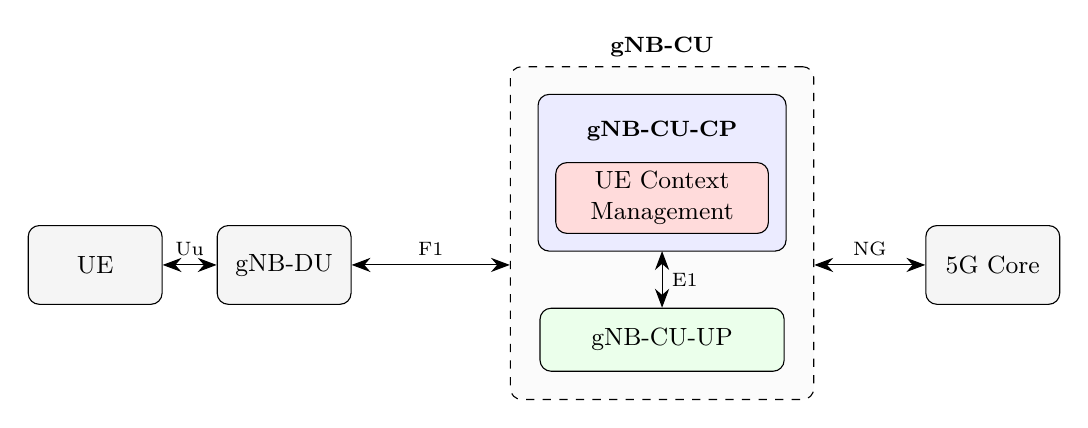
\begin{tikzpicture}[
    font=\small, >={Stealth[length=2.4mm]},
    box/.style={draw, rounded corners, minimum height=1.0cm, minimum width=1.7cm,
                align=center, fill=gray!8},
    cpbox/.style={draw, rounded corners, align=center, fill=blue!8},
    upbox/.style={draw, rounded corners, minimum width=3.1cm, minimum height=0.8cm,
                  align=center, fill=green!8},
    uecm/.style={draw, rounded corners, minimum width=2.7cm, minimum height=0.62cm,
                 fill=red!14, align=center}
  ]
  \node[box] (ue) at (0,0)   {UE};
  \node[box] (du) at (2.4,0) {gNB-DU};

  % Control plane, with UE Context Management shown nested inside it
  \node[font=\footnotesize\bfseries] (cpttl) at (7.2,1.7) {gNB-CU-CP};
  \node[uecm] (uecm) at (7.2,0.85) {UE Context\\ Management};
  % User plane
  \node[upbox] (up) at (7.2,-0.95) {gNB-CU-UP};

  % The background layer paints in source order and the central unit's fill is opaque, so
  % the control-plane box has to be drawn after it. Node (cp) carries the geometry that the
  % central unit and the E1 arrow are measured against.
  \begin{scope}[on background layer]
    \node[fit=(cpttl)(uecm), inner sep=6pt] (cp) {};
    \node[draw, dashed, rounded corners, fill=gray!3,
          fit=(cp)(up), inner sep=10pt, label={[font=\footnotesize\bfseries]above:gNB-CU}] (cu) {};
    \node[cpbox, fit=(cp), inner sep=0pt] {};
  \end{scope}

  \node[box] (core) at (11.4,0) {5G Core};

  \draw[<->] (ue) -- node[above,font=\scriptsize]{Uu} (du);
  \draw[<->] (du.east)         -- node[above,font=\scriptsize]{F1} (cu.west |- du);
  \draw[<->] (cu.east |- core) -- node[above,font=\scriptsize]{NG} (core.west);
  \draw[<->] (cp.south) -- node[right,font=\scriptsize]{E1} (up.north);
\end{tikzpicture}
\caption[Where the studied subsystem sits in the 5G NG-RAN]{Where the studied subsystem sits in the 5G NG-RAN. UE Context Management is
highlighted inside the gNB-CU-CP.\label{fig:ngran}}
\end{figure}

\section{Research gap}\label{sec:gap}
The RAN control plane has many threads and
tight latency bounds. Tail latency under too much load, not mean throughput, sets
the quality the network delivers. C++ gives the control and speed the domain
needs. But it leaves whole classes of memory and thread bugs to detection
at runtime. Rust promises to block those classes of errors at compile time at no
run-time overhead. It also offers a step-by-step adoption path through the C
application binary interface (ABI).

Five vendor-hosted Master's theses, all
done at Ericsson, have compared candidate languages for RAN and telecom
software. One weighs run-time cost against how fast people can build, across
C++, Rust, and Go~\cite{karlback2021ran}. One asks whether Rust could replace
C in RAN node management~\cite{olsson2023ranmgmt}. One builds a packet
processor, one thread per core, in async Rust. It measures that processor
against the Data Plane Development Kit (DPDK) program it
mirrors~\cite{olsson2023asyncpackets}. One measures median and p99 latency for
control-plane steps across five async
frameworks~\cite{arvidsson2025async}. The last builds matched C++ and Rust
versions of one program. That program turns a packed Abstract Syntax Notation
One (ASN.1) message back into a readable form. It compares
them with statistical tests~\cite{emberg2023asn1}. All five are directly
relevant. They do not all favour Rust. Olsson and Stenstr\"om's packet
processor reaches a fifth to a half of DPDK's throughput, with far worse
latency~\cite{olsson2023asyncpackets}. Arvidsson and Kaller's Rust p99 rises
more steeply past a threshold rate~\cite{arvidsson2025async}. Karlb\"ack and
Or\"o pick C++ where speed is critical. They still find Rust lightest on peak
memory~\cite{karlback2021ran}. Olsson's management software is as fast as C or
faster. It uses more peak memory~\cite{olsson2023ranmgmt}. Emberg and
Wadsten's pair is comparable in one session. It is $85$--$91\%$ worse in the
next~\cite{emberg2023asn1}.

Three of them change the language together with the run-time and the thread
model. A measured gap then cannot be blamed on the language rather than on the
framework~\cite{karlback2021ran,olsson2023asyncpackets,arvidsson2025async}.
In that packet-processor study the DPDK program does two to five times as much
work~\cite{olsson2023asyncpackets}. A compiler does not move throughput that
far. The run-time does. Olsson's management study and Emberg and Wadsten do
not change the run-time with the language~\cite{olsson2023ranmgmt,emberg2023asn1}. But they
report run time and peak memory, not tail latency under rising load. Emberg and
Wadsten come closest in method to this thesis. Their program keeps no state
between calls. The service in this thesis stores state and uses many threads.
Figure~\ref{fig:gapmap} places the five vendor theses beside the
general-purpose comparisons~\cite{pereira2017energy} and the matched
systems-software pairs~\cite{emmerich2019drivers,suchert2023stamp}. Each of
these groups leaves out at least one thing the figure asks for. No group keeps
the design fixed, measures the tail, and drives the service into overload.

The place these studies come from is part of the gap too. All five studies come from one
vendor. Their conclusions have never been tested against another
firm's software, targets or house rules. So what is known about this question
is what one firm's frameworks say about it. The published record on the other
side is thinner. There is no study of Rust among the indexed papers of the
vendor hosting this work. The nearest peer-reviewed stance from that side
argues for making memory-error sanitisation practical. It does not argue for
replacing it with a compile-time guarantee~\cite{gjomemo2016mesc}. That is the
strategy this thesis tests against.

\begin{figure}[ht]
\centering
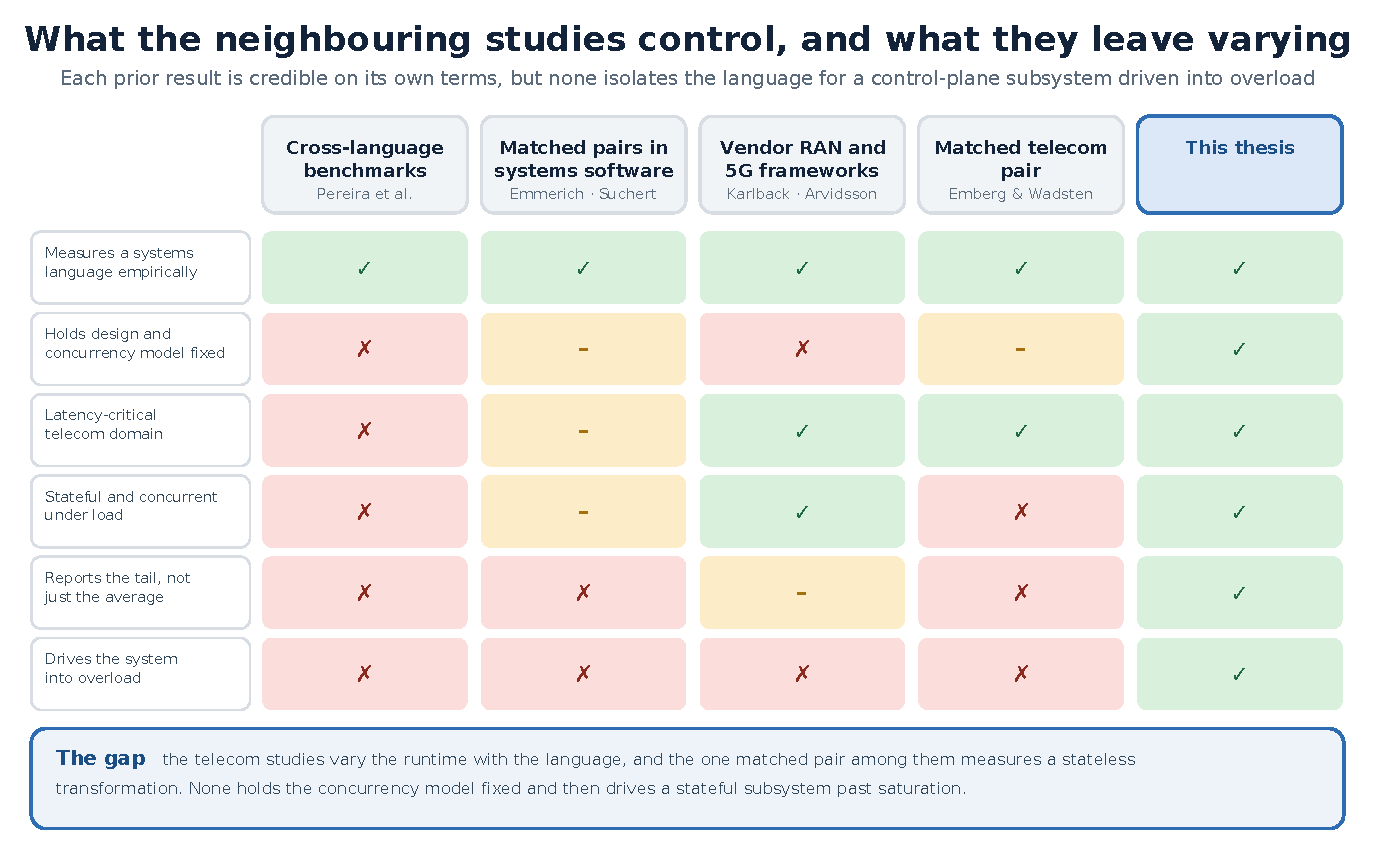
\includegraphics[width=\linewidth]{diagrams/pdf/29_research_gap.pdf}
\caption[A checklist of earlier comparisons]{A checklist of earlier comparisons. Each row is a
property a controlled answer would need, and each column is a group of studies.
The vendor-RAN column is the other Ericsson theses.
Emberg and Wadsten have their own column because they keep the design the same in both languages.\label{fig:gapmap}}
\end{figure}
% The figure fills the text block. Stretching the page to hold this
% paragraph pushed the last lines into the bottom margin, past where
% every other page stops. Break here so the paragraph stays whole on
% the next folio and this page ends on the same line as the rest.
\filbreak

What is missing from prior work is a direct, controlled test of a typical
control-plane part. The open questions are these. Does Rust hold its tail
latency under too much load against modern C++ when the thread model, operations, and
data layout stay fixed? Which bug classes does it remove, and at what stage
are the rest caught? What does its safety model cost in throughput and in CPU
and memory? What does step-by-step adoption cost in practice? Closing this gap
is the purpose of the four research questions. The next chapter grounds them
in the part under study, the bug classes, and the timing at stake. It also
sets out the method.


\chapter{Research Methodology\label{chapter:methodology}}
\chaptermark{Methodology}

The last chapter set out the gap. This chapter says how the study closes it.

\section{The UE Context Management subsystem}\label{sec:uecm}
The part under study is a UE Context Management service. Its operations follow the
UE-context lifecycle, RRC procedure execution~\cite{3gpp38331}, and mobility and
handover that the 3GPP design assigns to the control-plane part of a split gNB
(Section~\ref{sec:ranarch}). Figure~\ref{fig:fsm} shows the UE-context
lifecycle both versions encode the same way. The mixed workload of
Section~\ref{sec:workload} walks each UE through that machine.

\begin{figure}[ht]
\centering
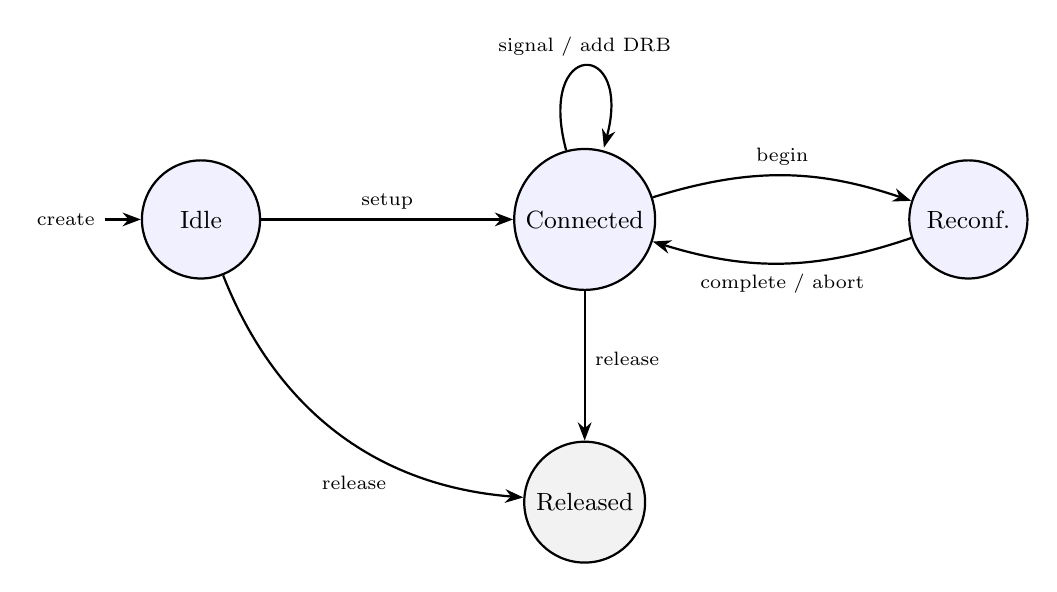
\begin{tikzpicture}[
    ->, >=Stealth, node distance=3.2cm, font=\small,
    every state/.style={draw, minimum size=1.5cm, fill=blue!6, thick},
    every edge/.style={draw, thick}
  ]
  \node[state, initial, initial text=\scriptsize create] (idle) {Idle};
  \node[state, right=of idle] (conn) {Connected};
  \node[state, right=of conn] (reconf) {Reconf.};
  \node[state, below=1.9cm of conn, fill=gray!10] (rel) {Released};

  \path (idle)  edge node[above,font=\scriptsize]{setup} (conn)
        (conn)  edge[bend left=18] node[above,font=\scriptsize]{begin} (reconf)
        (reconf) edge[bend left=18] node[below,font=\scriptsize]{complete / abort} (conn)
        (conn)  edge node[right,font=\scriptsize,pos=0.45]{release} (rel)
        (idle)  edge[bend right=32] node[below=8pt,font=\scriptsize,pos=0.55]{release} (rel);
  \path (conn) edge[loop above] node[font=\scriptsize]{signal / add DRB} (conn);
\end{tikzpicture}
\caption[UE-context lifecycle state machine]{UE-context lifecycle state machine.
Operations invalid for the current state return an error instead of changing
state.\label{fig:fsm}}
\end{figure}

UECM is core RAN layer-3 work. It has the traits that make live control-plane
code hard. Each UE has state that changes, the operation lifecycle is strict,
and many UEs run at once. Delay targets are the ones the 5G system sets for
control-plane procedures~\cite{3gpp38913,3gpp22261}. Findings about how a language
handles those traits are most relevant to other stateful, multi-thread
control-plane services of this kind. The part is also small enough to specify in full and build twice.
That is what makes a parity-tested comparison possible.

The interface is small and built around the lifecycle. It can create and
release a context, set up a connection, handle an in-session signalling
message, add a data radio bearer, begin, complete, or abort a
reconfiguration, and look up a context's state under load. Each
operation is defined for each state of Figure~\ref{fig:fsm}. An illegal operation
returns a typed error and leaves the context unchanged. That closed set lets
the same tests and the same workload drive both versions along the same
paths.

RQ2 needs a catalogue, not a loose list of hazards. One is built from this
operation set: $\FaultClasses$ classes in two groups of seven. Seven come from inside
the region safe Rust claims to govern. Seven were chosen because safe Rust is
expected not to prevent them. Each has its expectation recorded before the
programs were run. Section~\ref{sec:safetyresults} reports what each one did.

The tail is the metric because of two traits of this part. One user-visible
action, a call setup or a handover, becomes many dependent control-plane
operations. The slowest member gates completion. A busy site drives thousands of
such procedures per second. So a far-tail point is reached often enough to
matter. The failure shape is the second reason. Under an open-loop clock,
achieved rate can track offered load until either the service or timed
producer work becomes limiting. Latency then rises sharply. That is why this
study sweeps past the apparent saturation point and audits what the timed
path contains.

\section{Research approach}\label{sec:approach}
The study runs experiments. It also builds the thing it measures: a matched
pair of versions, plus the harness that drives them. Both are built from one
frozen spec. Evidence comes from three separate methods: a load sweep contributes to
RQ1 and RQ3, controlled fault injection answers RQ2, and an FFI migration
prototype answers RQ4. A weakness in one of them, such as how much the host
can move the tail, does not carry into the rest of the claims.

Each question asks how one outcome depends on one variable, the language. The
language has to be the only planned gap between the two objects under test.
That rules out the most common way to compare languages. In that form two
programs written on their own are measured, and the gap is taken to be the
language. Such a gap also carries the design, the libraries, and the skill of
their authors. Building both sides from one spec removes that confound. Where
a question can be answered with numbers, it uses numbers. Where it cannot, the
answer is still by a fixed plan, in words. That is how this study treats the
kind of guarantee in RQ2. RQ4 asks about the design cost of the application
programming interface (API).

The closest prior work is the five vendor-hosted theses of
Section~\ref{sec:gap}. They appear in no citation database. They had to be
found by searching each university's own archive by hand. The same searches
found no Finnish thesis on Rust in a radio-access setting. They found no
indexed paper mentioning Rust from the vendor hosting this work. The search
returned no study that measures the tail of a Rust and a C++ version of the
same stateful, multi-thread control-plane part under too much load.

Table~\ref{tab:design} maps each research question to the method, artefact,
data and metric that answer it. RQ1 and RQ3 share H1, worded to cover a speed
tie in both the latency and the resource sense. That wording turns out to be the
hypothesis's main weakness. RQ2 does not depend on the host. RQ4 depends on it
along one axis. Build time is a timing. So it is read as a ratio between two
toolchains measured in turn on one machine.

\begin{table}[ht]
\centering
\small
\caption[How each research question is answered]{How each research question is
answered. RQ1 and RQ3 carry two methods rather than one. Below saturation the
sweep measures the round-trip a deployment would experience. The split of the
core from the handoff measures the part the language can own, while a
same-host control tests whether high-load recorder work contaminates the sweep.
\label{tab:design}}
\renewcommand{\arraystretch}{1.2}
\setlength{\tabcolsep}{4pt}
\begin{tabular}{@{}p{0.07\linewidth} p{0.27\linewidth} p{0.27\linewidth} p{0.27\linewidth}@{}}
\hline\hline
RQ & Method & Artefact / data & Primary metric \\
\hline
RQ1 & Load sweep to overload, interleaved repeats & Benchmark harness, latency histograms &
median, p99/p99.9/p99.99, and maximum vs.\ offered load \\
RQ3 & Same sweep, resource capture & \texttt{getrusage} samples per run &
peak resident set size (RSS), CPU, throughput \\
RQ1, RQ3 & Core called directly, then through the service &
Matched microbenchmark pair &
operation vs.\ cross-thread handoff \\
RQ2 & Controlled fault injection & Defect catalogue, three C++ sanitisers,
\texttt{rustc}, Loom/Shuttle, Miri &
compile-time / runtime / undetected \\
RQ4 & FFI migration prototype & C++ host $+$ Rust C-ABI boundary &
boundary size, \texttt{unsafe} scope, per-call cost \\
\hline
\end{tabular}
\end{table}

\section[Methods per research question]{Methods per research question, in outline}\label{sec:methodbrief}
RQ1 and RQ3 are studied with an open-loop load sweep from light load to well
past saturation. Open-loop means the generator keeps to its send schedule
instead of waiting for replies~\cite{schroeder2006openclosed}. The four build
variants are interleaved inside each repeat. A second timing splits the core operation
from the cross-thread handoff around it. The end-to-end round-trip bundles two
costs of two kinds. Only one of them can differ between the languages. A third
timing takes the contended queue and the reply handle on their own. A
same-host control then writes the histogram fill after the timed window,
holding the pin and \texttt{nohz\_full}. That control isolates the fill.
Clock A, which drops the fill, was not repeated on this host.

RQ2 is answered by controlled fault injection~\cite{natella2016fault}. Each
defect class is a small program of its own in both languages.
The C++ side is built and run under AddressSanitizer. It is also run under
ThreadSanitizer and UndefinedBehaviorSanitizer. The safe-Rust side is compiled
and, where it compiles, run under a bounded timeout. No static analyser is
run, on purpose.
The C++ columns then report the tooling this study ran. They do not report a
ceiling on what C++ tooling could find. RQ4 is answered by a working
prototype in the direction a real migration takes. A C++ host calls an
unchanged Rust core across a C ABI. This boundary is called the FFI seam here.
It is the thin layer that converts between the C++ host and the Rust core.
The per-call cost is measured on a real
operation and not inferred from an empty crossing. Memory bugs that cross a
language sit at that seam~\cite{li2022crosslang}.

\section{Fairness as a controlled variable}\label{sec:controlsbrief}
A language comparison is only as good as the variables it holds fixed. The
spec is frozen before either version exists. The thread model, the allocator
and its arena count, the opt level, the hash function, the histogram method
and the load schedule are matched across the two sides. They are never tuned
per side. Where the two languages could not be written alike, the gap is
logged instead of resolved. The two sides are shown to match by diffing match
logs operation by operation. For a given seed they also execute the same
operation order. The four variants take turns on the same pinned cores
inside each repeat. That keeps recent cache contents and recent branch
guesses close, because the same work runs one after another. The test does
not empty the cache between variants. It also does not first train the CPU
on those branches. It holds the work and the cores fixed. It does not hold
the CPU's recent memory and branch history fixed.

\section{Statistical treatment}\label{sec:statsbrief}
The statistical design is fixed in advance. The family of tested comparisons is
listed ahead of the campaign. So a load picked after seeing a sweep cannot
enter it. Each comparison is an exact paired permutation test over \NRepeats{}
interleaved repeats, with a bootstrap confidence
interval~\cite{efron1993bootstrap}, Holm-corrected across the
family~\cite{holm1979simple}. The floors the test can reach ($\MinAttainableP$
uncorrected, $\CorrectedFloor$ corrected) are quoted so that a null can be
told apart from a math limit. Representative-load throughput is reported but
not tested because it is pinned to the offered rate. Jitter is outside the
research questions. The maximum is too sensitive to one disturbed operation
for pairing to rescue it. The pooled p99.99 far tail has the operation as its
unit, so it has no across-repeat interval to test. No latency percentile is
tested after saturation because cumulative schedule drift makes it a lower
bound rather than a service-time estimate.

\section{Reproducibility and research artefacts}\label{sec:repro}
A third party can rebuild the results without access to Nokia's private code.
The versions are driven entirely by the public frozen spec. The benchmarking
harness, the fault catalogue and its runner, and the FFI prototype are
published with the thesis. Each plot of measured data is rebuilt by one
script from the raw logs. So is each quoted number in the results. The script
is \texttt{bench/refresh\_thesis.sh}. That claim does not cover the hand-drawn
schematics, which explain a concept rather than report a result. And running
the same scripts over another host's campaign rebuilds the artefacts by the
same procedure, not with the same values.

The logs that script reads are part of the package. Each campaign has its own
script and its own macro prefix, so a figure from one cannot reach a sentence
about another. Each run's host setup is recorded and stored beside the
campaign data. Nothing in the results chapters is typed from those files by
hand.

\chapter{Design and Implementation\label{chapter:design}}
\chaptermark{Design}

Nothing is built until the spec is frozen. It fixes the public API, the UE
state machine, the data layout and the steps on it, the locks and shard size,
and the thread model. Both versions follow it. The test then times the
language, not a gap of design or of skill. The spec is itself an output of the
study. It is the main control against writer bias.

One thread model is used on both sides: shared-nothing and thread-per-shard.
That layout is known to change tail latency by
itself~\cite{enberg2019threadpercore}. The layout is held fixed as a fairness
control. A production gNB-CU-CP schedules UE work differently. The id space is split into shards. Each
shard is owned by one worker thread. That thread alone reads or changes it.
So no lock guards context state. Callers send a request to the owning shard's
bounded queue. They wait on a one-shot reply handle. The queue blocks when it
is full. That is on purpose. A drop rule would hide overload. This study needs
overload to show up as latency. The only shared mutable state either version
allows is one atomic counter. No control flow depends on its value.
Figure~\ref{fig:arch} shows the data flow. There is one multi-producer,
single-consumer (MPSC) queue per shard. Its worker drains it first in, first
out (FIFO).

\begin{figure}[ht]
\centering
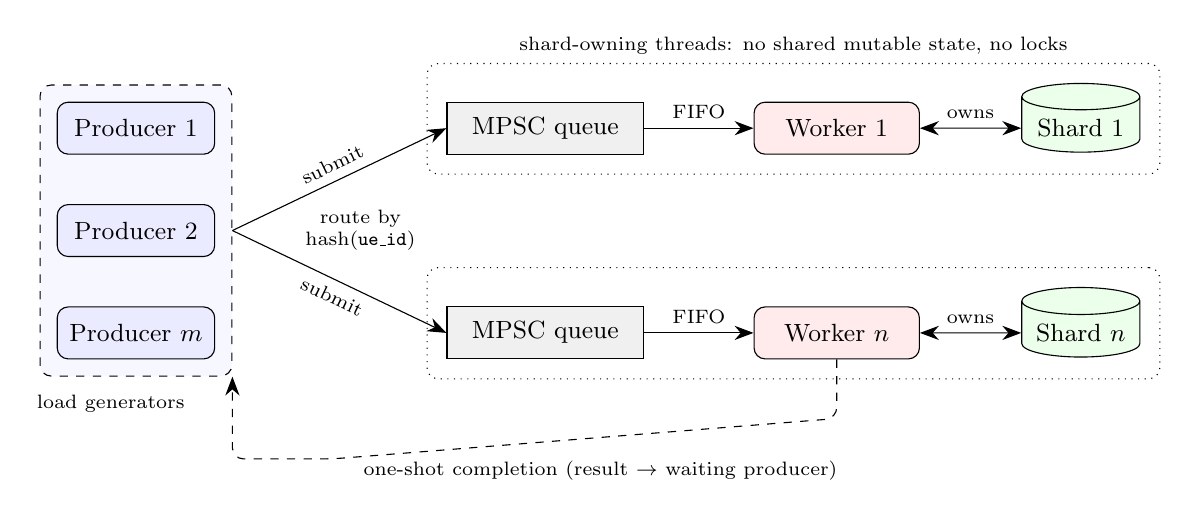
\begin{tikzpicture}[
    font=\small,
    prod/.style={draw, rounded corners, minimum width=2.0cm, minimum height=0.66cm, fill=blue!8},
    queue/.style={draw, minimum width=2.5cm, minimum height=0.66cm, fill=gray!12},
    worker/.style={draw, rounded corners, minimum width=2.1cm, minimum height=0.66cm, fill=red!8},
    store/.style={draw, cylinder, shape border rotate=90, aspect=0.25, minimum width=1.5cm, minimum height=0.85cm, fill=green!8},
    lane/.style={draw, dotted, rounded corners, inner sep=7pt},
    >={Stealth[length=2.4mm]}
  ]
  \node[prod] (p1) at (0,1.3)  {Producer 1};
  \node[prod] (p2) at (0,0.0)  {Producer 2};
  \node[prod] (p3) at (0,-1.3) {Producer $m$};
  \begin{scope}[on background layer]
    \node[draw, dashed, rounded corners, fill=blue!3, fit=(p1)(p2)(p3), inner sep=6pt] (pg) {};
  \end{scope}
  \node[font=\scriptsize, anchor=north] at ([xshift=-0.32cm,yshift=-3pt]pg.south) {load generators};

  \node[queue] (q1) at (5.2,1.3)   {MPSC queue};
  \node[worker](w1) at (8.9,1.3)   {Worker 1};
  \node[store] (s1) at (12.0,1.3)  {Shard 1};
  \node[queue] (qn) at (5.2,-1.3)  {MPSC queue};
  \node[worker](wn) at (8.9,-1.3)  {Worker $n$};
  \node[store] (sn) at (12.0,-1.3) {Shard $n$};
  \begin{scope}[on background layer]
    \node[lane, fit=(q1)(s1)] (lane1) {};
    \node[lane, fit=(qn)(sn)] (lanen) {};
  \end{scope}
  \node[font=\scriptsize] at (8.35,2.35) {shard-owning threads: no shared mutable state, no locks};

  \node[font=\scriptsize, align=center, fill=white, inner sep=2pt] at (2.85,0) {route by\\ hash(\texttt{ue\_id})};
  \draw[->] (pg.east) -- (q1.west) node[midway, above, sloped, font=\scriptsize]{submit};
  \draw[->] (pg.east) -- (qn.west) node[midway, below, sloped, font=\scriptsize]{submit};

  \draw[->]  (q1) -- node[above, font=\scriptsize]{FIFO} (w1);
  \draw[->]  (qn) -- node[above, font=\scriptsize]{FIFO} (wn);
  \draw[<->] (w1) -- node[above, font=\scriptsize]{owns} (s1);
  \draw[<->] (wn) -- node[above, font=\scriptsize]{owns} (sn);

  \draw[->, dashed, rounded corners=4pt]
      (wn.south) -- ++(0,-0.75) -- (2.5,-2.9) -| (pg.south east);
  \node[font=\scriptsize] at (5.9,-3.05) {one-shot completion (result $\rightarrow$ waiting producer)};
\end{tikzpicture}
\caption[Shared-nothing, thread-per-shard architecture]{Shared-nothing,
thread-per-shard architecture. Producers submit to a bounded MPSC queue per
shard, and that shard's worker drains it.\label{fig:arch}}
\end{figure}

Fairness is kept below the design as well as in it. Both builds link the same
\texttt{jemalloc}. Both keep a system-allocator build as a control. Both
compile at the same opt level. Both record latency through one high-dynamic-range
(HDR) histogram set up the same way~\cite{tene_hdrhistogram}. Hashing is pinned
on both sides. SplitMix64 assigns the shard~\cite{steele2014splitmix}. FNV-1a, the
Fowler--Noll--Vo hash~\cite{rfc9923}, is used inside the map. C++'s default hash of an
integer is often just the number itself. Rust's is strong on purpose. Left as they came,
the two standard libraries would have been the measurement.

Where the languages cannot meet a need the same way, the gap is written into a
forced-idiom log and then measured. Two of those gaps were candidates for the
campaign-clock overload result of Section~\ref{sec:overload}. One is the bounded queue. Rust takes it
from \texttt{sync\_channel}. C++23 still has no such primitive, so C++ builds
one from a mutex and two condition variables. The other is the reply handle,
\texttt{std::promise} against a fresh \texttt{mpsc} channel per request. Tests
of those primitives and a replacement reply handle were run on an earlier
host. They do not explain the smaller lead that remains on this one once the
fill moves. A
third carries the core-operation result of Section~\ref{sec:perfresults}: the
per-shard container is each language's own standard hash map. A fourth is the
request encoding. C++ has no payload-carrying enumeration in this idiom, so a
request becomes a tagged struct holding each field any operation might need,
$\CppRequestBytes$~bytes against Rust's $\RustRequestBytes$. The net result is
a Rust core $\NlocRise\%$ longer in code lines. Its branching complexity is
$\CcnTotalDrop\%$ lower~\cite{lizard}. The Rust library contains no
\texttt{unsafe} at all.

Parity is tested and not assumed. Language-neutral vectors run in both
versions. Their logs are diffed operation by operation. A cross-diff cannot tell ``both
correct'' from ``both wrong in the same way''. A third version in Python acts
as an independent oracle. It has to reproduce all $\ConfHandOps$ hand-derived
expectations before it may generate any of its own. A campaign of
$\ConfGenOps$ generated operations found no mismatch. The C++ side runs under
AddressSanitizer, ThreadSanitizer and UndefinedBehaviorSanitizer. The Rust
side runs under Miri. A clean sanitiser result is bounded by the code that
actually ran.

\chapter{Experimental Setup and Evaluation\label{chapter:eval}}
\chaptermark{Evaluation}

This chapter starts with the test hosts and the work they run. Results then
follow by load, then by the rest of the questions.

\section{Testbed setup\label{sec:testbed}}
Some numbers in this chapter come from the tools and the code. Other
numbers depend on the host they ran on. The reported campaign comes from
one bare-metal host, a single-socket \MainCpu{}. Each core runs one
thread. Extra threads on a core are \MainSmt{}. The host runs
\MainHostDistro{} on kernel \MainKernel{}. Linux can raise and
lower each core's clock as load and heat change. The clock is held
fixed. The governor is \MainGovernor{}, and boost is off. The
test may use only cores \MainPinned{}. There is no hypervisor. The
program runs on the host itself, not inside a virtual machine. On those
cores the kernel turns off its timer tick (\texttt{nohz\_full}).
If left on, those ticks would show up in the latency numbers. The study does
not use \texttt{isolcpus}. That flag also stops the kernel sharing work
across the allowed cores. Each test thread then lands on one core.

The build tools are not the ones on the host. Both sides are built
and run inside an image that carries \MainDistro{} with
\texttt{g++~\MainGpp} and \texttt{rustc~\MainRustc}. The image pins the
\texttt{gcc-toolset} major and not the point release. The earlier
sweep on a virtual machine then built with \texttt{g++~\GuestGpp},
one GNU Compiler Collection (GCC)~15 release earlier. An image still uses the kernel of the host
it sits on. The two sweeps then differ in the hardware, in the kernel
(\MainKernel{} against \GuestKernel{}), and in that compiler release.

Until late in the work the sweep ran on a Kernel-based Virtual Machine (KVM)
on an \GuestCpu{}, with none of the core controls above. The capture records
the hypervisor as \GuestVirt{}, the guest userland as \GuestDistro{}, and the
guest kernel as \GuestKernel{}. On that
host the $95\%$ band on one variant's p99 spans
$\GuestPNineNineMaxCI\,\mu$s. The four variants' p99 values differ by
$\GuestPNineNineRange\,\mu$s. The noise on one variant was larger than the gap
between all four. That sweep is kept. It uses the same design as
this one. The two can then be set next to each other to ask which findings belong to the code.
A third sweep on a second bare-metal \BmCpu{} uses a new shard count, load
grid, run count and tools. It tests whether the findings hold under those
changes as a set, not any one of them on its own.
Appendix~\ref{appendix:config} itemises the three hosts and the campaign
parameters field by field.

\section[Workload and measurements]{Workload and measurements\label{sec:workload}}
The work is made for the test. The steps it takes come from the 3GPP
rules~\cite{3gpp38401,3gpp38331}. A driver that always sends the same
steps walks each UE through the connection lifecycle those rules
define. The \emph{signal} work first connects a set of UEs, then sends the
same signal call again and again. That picks out the common path. The
\emph{mixed} work walks each UE through context creation, setup,
signal, bearer setup, reconfiguration or handover, and release. A fixed
random order makes both sides see the same counts of each call kind
for a given seed. That is also a check that the two sides did the same
work. Figure~\ref{fig:workload} shows the two loads and the steps the
mixed one walks.

\begin{figure}[ht]
\centering
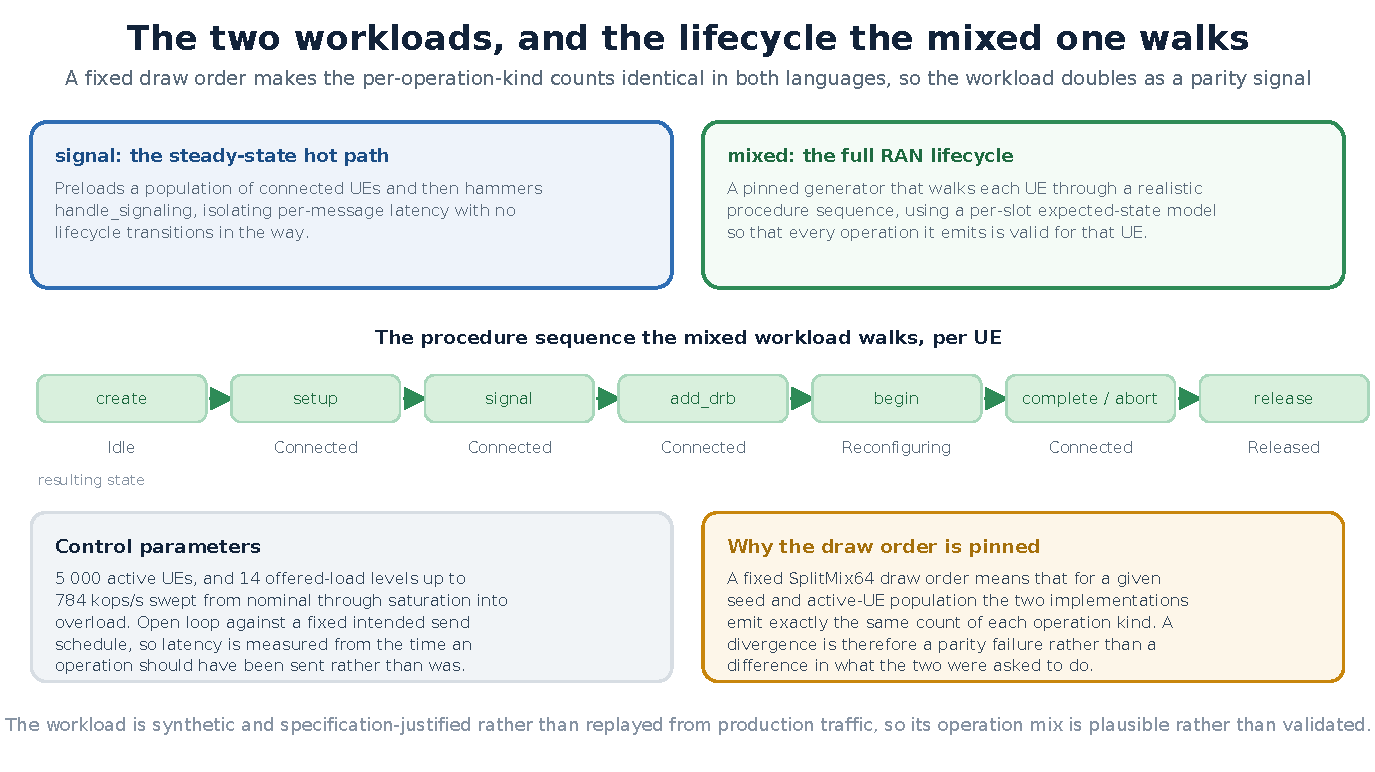
\includegraphics[width=0.78\linewidth]{diagrams/pdf/27_workload_timeline.pdf}
\caption[The two test workloads]{The two
workloads, and the lifecycle the mixed one walks. Signal repeats the common
path, and mixed walks each UE through the procedure sequence drawn
below.\label{fig:workload}}
\end{figure}

The steps match the 3GPP rules. Those rules do not set the mix.
A real cell's handover rate rests on the site and the
time of day, and no public figure fixes it. A mix that does not match a real
cell moves both sides by the same amount. It limits how far the numbers
travel. It does not make the test unfair. The sender keeps to its
plan even if the service is late (open-loop). The histogram is
corrected so a stall does not hide missing replies (coordinated-omission
bias)~\cite{schroeder2006openclosed,tene_hdrhistogram}. Each load is
run \NRepeats{} times. The four language and heap variants are interleaved
inside each run. Each point is a median with a bootstrap $95\%$
band~\cite{georges2007rigorous,efron1993bootstrap}.

The load used for the resource plots is $\ReprLoad$~kilo-operations per second
(kops/s). It is a chosen
value, not one made from the sweep. The first rule this study used was the
peak load whose p99 stayed under $5$~ms. On the virtual machine that rule
landed on the noise of the host. On a quiet host it climbs until the service
can no longer keep up. It is kept only as a check. The lowest finished rate
among the four variants is $\SatKnee$~kops/s, reached when the sent
load is $\TrackingLoad$~kops/s.

\section{Results}
The safe code results and most of the migration results do not depend on which
host was used. The speed and RSS results do. Each figure below was
timed on the host of Section~\ref{sec:testbed} unless the caption says
so.

\subsection{Below saturation (RQ1, RQ3)}\label{sec:perfresults}
At the representative load of $\ReprLoad$~kops/s, where every variant keeps
up with the sent load, the four variants'
medians lie within $\PFiftyRange\,\mu$s of each other, $\PFiftySpread\%$. A
paired test still finds a gap of $\PFiftyDiffAbsMax\,\mu$s in Rust's
favour under both heaps. Figure~\ref{fig:loadsweep} shows the sweep behind
that. Higher tails can now be read as well. The widest band on
one variant's own p99 spans $\PNineNineMaxCI\,\mu$s. The four variants' p99
values differ by $\PNineNineRange\,\mu$s. So the noise on one is smaller than
the gap between them. On the virtual machine the same two sizes were
$\GuestPNineNineMaxCI\,\mu$s against $\GuestPNineNineRange\,\mu$s, the other
way around. Both p99 rows and both p99.9 rows clear the Holm correction,
\NTailSignificant{} rows in all, in the same way as the median.
Table~\ref{tab:latency} reports p99.9 and the maximum at the chosen
load. The maximum is kept out of the tested family, as the pooled p99.99 is.

\begin{table}[ht]
\centering
\small
\caption[Per-operation latency at the representative load]{Per-operation latency,
in microseconds, at $\ReprLoad$~kops/s. The median over \NRepeats{} repeats sits
above its bootstrap $95\%$ interval. $^{\dagger}$The p99.99 column is pooled across
repeats, so it has no interval. The maximum has a repeat-wise interval but stays
outside the tested family because one disturbed operation can determine it.
\label{tab:latency}}
\LatencyTabular
\hline\hline
\LatencyHead \\
\hline
C++ (system alloc) & \mci{217.2}{163.8}{237.2} & \mci{355.1}{289.3}{389.4} & \mci{674.3}{395.3}{1538.0} & \mci{2170}{910}{5594} \\
C++ (jemalloc) & \mci{225.8}{181.1}{261.2} & \mci{410.1}{305.7}{11280.4} & \mci{1188}{544}{14213} & \mci{3590}{1472}{16291} \\
Rust (system alloc) & \mci{214.3}{191.6}{238.8} & \mci{376.3}{330.2}{3629.1} & \mci{1068}{504}{6955} & \mci{2404}{1129}{9667} \\
Rust (jemalloc) & \mci{208.4}{193.7}{223.1} & \mci{388.9}{342.3}{478.0} & \mci{763.4}{479.5}{4272.1} & \mci{2804}{1114}{7606}
\\
\hline
\end{tabular}
\end{table}

\begin{figure}[ht]
\centering
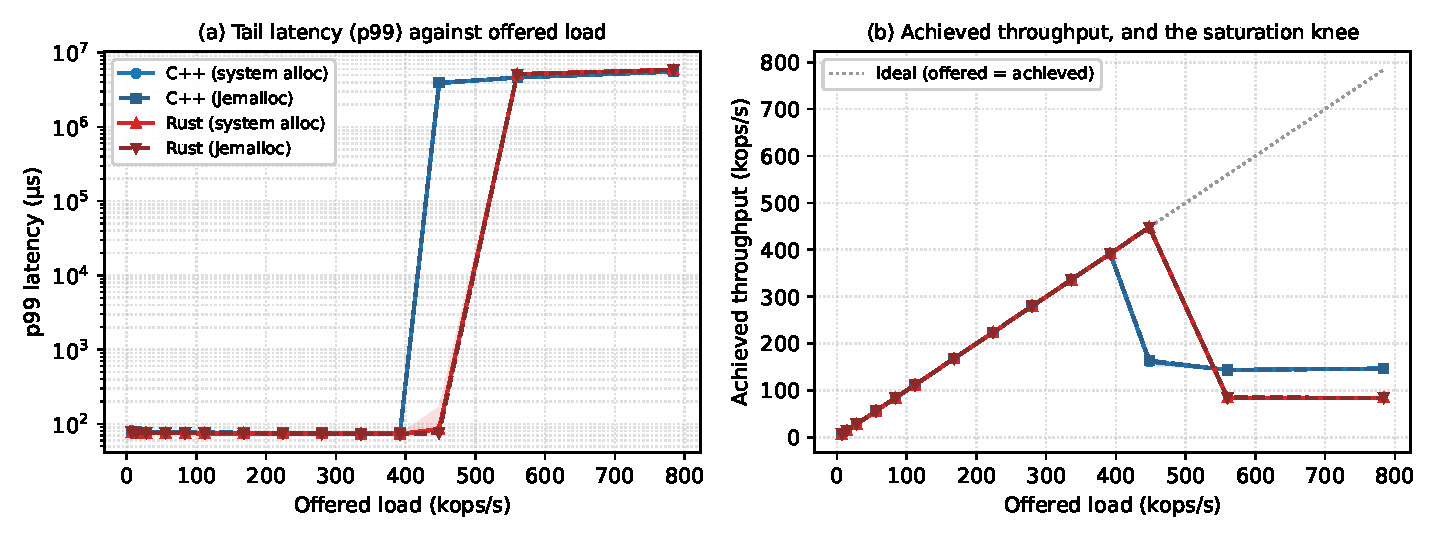
\includegraphics[width=\linewidth]{figures/fig_load_sweep.pdf}
\caption[The load sweep: tail latency and achieved throughput]{Panel (a) is
p99 below the knee, on one linear scale, through $\TrackingLoad$~kops/s.
The four variants sit within a few microseconds, so they are drawn together.
In (b) and (c) each variant has its own panel. Panel (b) is the tail on a
log scale across the whole sweep. Panel (c) is achieved throughput, and the
dotted line matches the offered load. Lines are medians over \NRepeats{}
repeats, and the bands in (b) and (c) are bootstrap $95\%$ confidence
intervals.\label{fig:loadsweep}}
\end{figure}

The far tail can be read here too. The runs' histograms are pooled, which
gives \FarTailSamplesMin{} to \FarTailSamplesMax{} calls per variant. The
two \FarTailLower{} variants sit below both C++ variants. The widest pair
differs by $\FarTailRange\,\mu$s. The slowest Rust variant still sits
$\FarTailLangSep\,\mu$s below the fastest C++ one. A second bare-metal host at another shard count agrees,
running $\BmFarTailCppLo$--$\BmFarTailCppHi\,\mu$s for the C++ variants against
$\BmFarTailRustLo$--$\BmFarTailRustHi\,\mu$s for the Rust ones, and the ranges do not meet.
A second limit does not come from the host. No host would remove it. An
end-to-end round-trip spends only $\BudgetCoreShareMax\%$ of its time on the
work the language does. The rest is passing the request to another thread,
and that time is charged to the operating system. When the work inside the
language is this small, time spent crossing from thread to thread
dominates~\cite{zhou2025oltp}. Figure~\ref{fig:e2eclock} draws that split.
This sweep cannot bound a language effect
either way, which Figure~\ref{fig:budget} sets beside what the sweep can
still show. Timed on its own, the core call is $\BudgetCoreRatio\times$
faster in \BudgetCoreFaster{}. The test does not trace the cause. The stock
hash map is one candidate. Compiler code generation may also own part of the
gap.

\begin{figure}[ht]
\centering
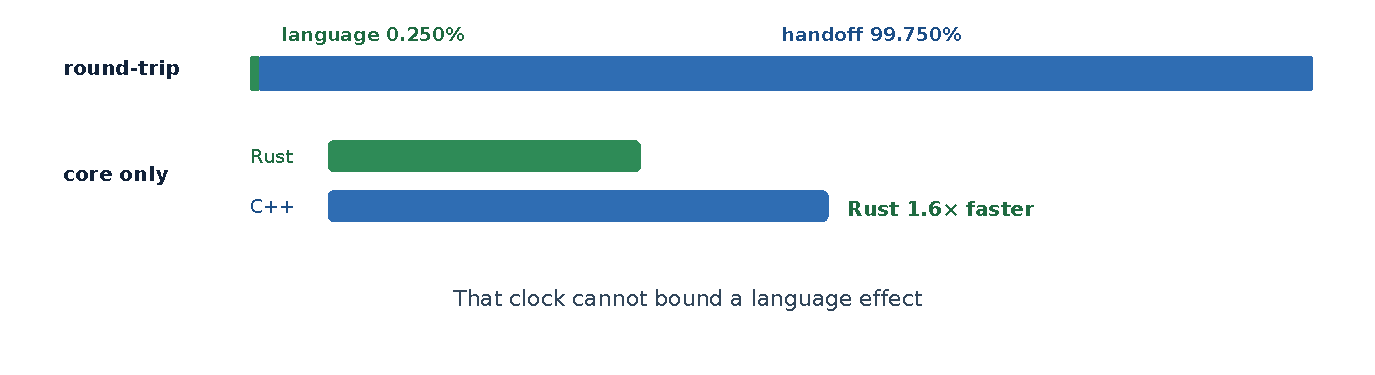
\includegraphics[width=\linewidth]{diagrams/pdf/31_e2e_clock.pdf}
\caption[Where the end-to-end clock goes]{Where an end-to-end
round-trip's clock goes. The language share is
$\BudgetCoreShareMax\%$. A clock that spends the rest on handoff cannot bound
a language effect.\label{fig:e2eclock}}
\end{figure}

\begin{figure}[ht]
\centering
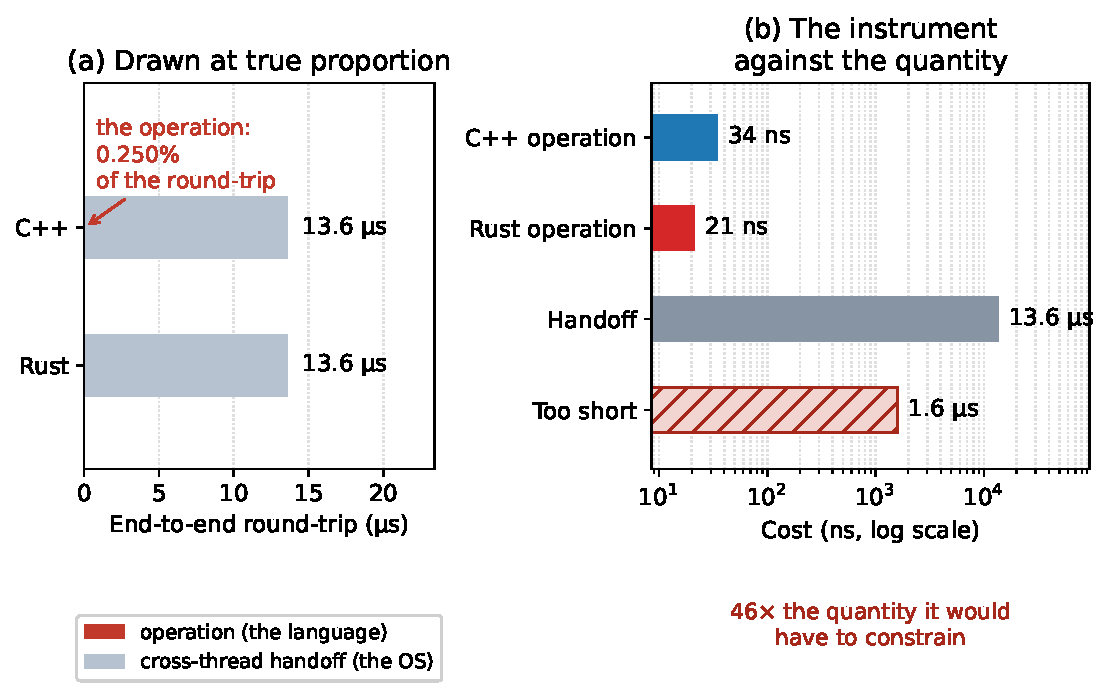
\includegraphics[width=\linewidth]{figures/fig_budget_thesis.pdf}
\caption[How small the language’s share of a round-trip is]{Where
an end-to-end round-trip's cost goes. \textbf{(a)} The round-trip at true
proportion. \textbf{(b)} Both operation measurements sit inside the sweep's
blind zone by a factor of $\BudgetBoundVsCore$.\label{fig:budget}}
\end{figure}

\subsection{Past saturation (RQ1)}\label{sec:overload}
Under the campaign clock both languages keep up through
$\TrackingLoadCpp$~kops/s and $\TrackingLoadRust$~kops/s, the same load.
At $\KneeSplitLoad$~kops/s the split is inside Rust. The \KneeSplitKeepHeap{}
heap still serves $\KneeSplitMedKeep$~kops/s. The \KneeSplitDropHeap{} median
is $\KneeSplitMedDrop$, and $\KneeSplitMeet$ of $\KneeSplitRepeats$ repeats
on that heap still meet the offered rate. That rung was found after the data
and is shown, not tested.
Figure~\ref{fig:loadmap} maps the representative load, the shared tracking
load, the allocator split, and the overload point.

\begin{figure}[ht]
\centering
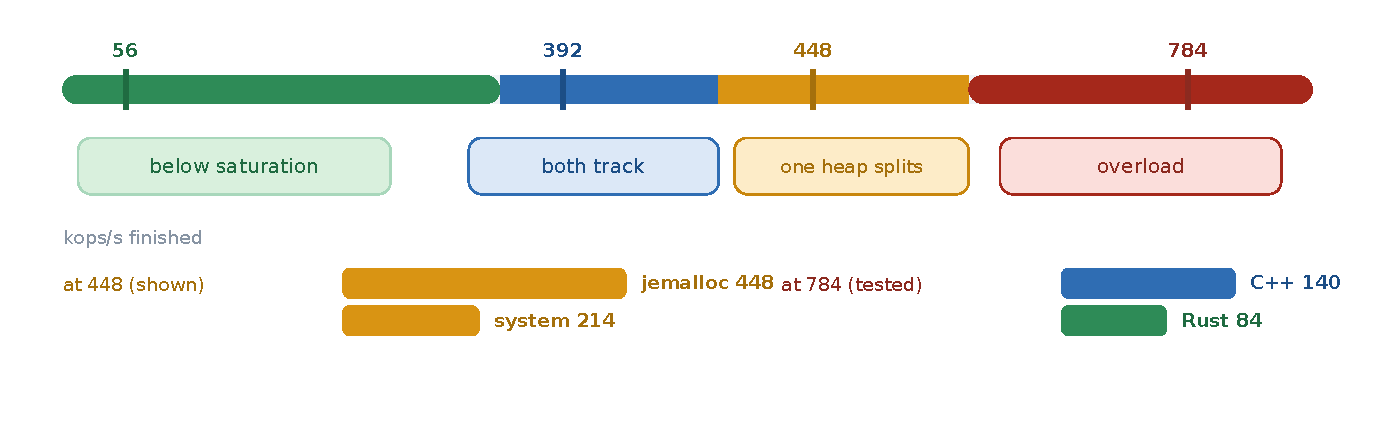
\includegraphics[width=0.78\linewidth]{diagrams/pdf/30_load_regimes.pdf}
\caption[Four load points, from a light load to overload]{Four load points, from a light load to overload. Operating points on
the offered-load axis, spaced for reading, not to scale. Ticks are
$\ReprLoad$, the shared tracking load $\TrackingLoad$, the allocator split at
$\KneeSplitLoad$, and $\OverloadLoad$~kops/s. Bars at the split are the two
Rust heaps on the campaign clock. Bars at $\OverloadLoad$ are the two
languages, also on that clock.\label{fig:loadmap}}
\end{figure}

Deeper, at $\OverloadLoad$~kops/s sent, \OverloadSustainedFaster{} still
finishes $\OverloadThrCpp$~kops/s where \OverloadSustainedSlower{} finishes
$\OverloadThrRust$, a factor of $\OverloadThrRatio$, in \OverloadThrAgree{}
runs under both heaps. The Holm-corrected $p$ is as small as this test family
can go. The slower variant uses $\OverloadCpuPerOpRatio$ times the CPU for
each call it finishes. That quantity belongs to the whole campaign process,
including the recorder, and does not identify service work.

Clock B repeats the same grid on this host, over $\ProbeAfterRuns$ runs.
The processor is \ProbeAfterCpu{}, the pin is \ProbeAfterPinned{}, and
\texttt{nohz\_full} is \ProbeAfterNohzFull{}. Those match the campaign.
Only the fill moves, to after the timed window. When a sender falls behind,
the harness still writes up to $\ProbeAfterCap$ extra samples for each
finished call, but it writes them outside the window. Clock A was not
repeated here. It remains an earlier host. Its percentiles stay
coordinated-omission biased, so they are not an RQ1 tail result.

Moving the fill removes both campaign patterns. At $\KneeSplitLoad$~kops/s,
C\texttt{++} serves $\ProbeAfterKneeThrCpp$~kops/s and Rust serves
$\ProbeAfterKneeThrRust$. Rust still tracks to $\ProbeAfterTrackRust$~kops/s
and C\texttt{++} to $\ProbeAfterTrackCpp$. At the top load Rust is ahead on
both heaps. On the system allocator C\texttt{++} finishes
$\ProbeAfterThrRatioSystem$ of Rust's throughput, $\ProbeAfterThrCppSystem$
against $\ProbeAfterThrRustSystem$~kops/s, at $p \ProbeAfterThrPSystem$.
Under \texttt{jemalloc} the figure is $\ProbeAfterThrRatioJemalloc$,
$\ProbeAfterThrCppJemalloc$ against $\ProbeAfterThrRustJemalloc$, at
$p \ProbeAfterThrPJemalloc$. These tests sit outside the pre-committed Holm
family.

What remains is that smaller Rust lead. CPU per completed operation on the
deferred plateau is $\ProbeAfterCpuPerOpRatio$, with
\ProbeAfterCpuPerOpHigher{} the higher one, against $\OverloadCpuPerOpRatio$
while the fill ran inside the window. The large ratio is the recorder. The
smaller lead is not that ratio. This visit took no allocation profile, so
the lead is reported and not explained. Queue and channel substitutions from
an earlier host do not explain it either. Percentiles on Clock B are
schedule drift, not service time. The campaign stays the pre-committed
compared pair. Figure~\ref{fig:overload} compares both clocks on this host
and keeps the two heaps apart.

\begin{figure}[ht]
\centering
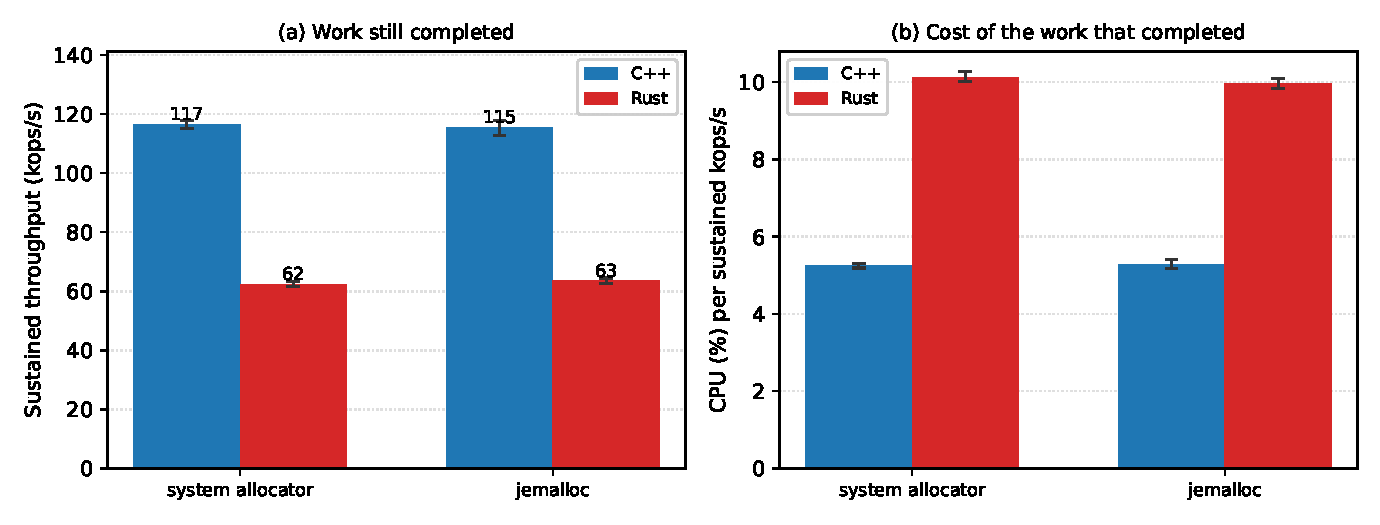
\includegraphics[width=\linewidth]{figures/fig_overload.pdf}
\caption[Campaign and deferred-fill throughput on this host]{Throughput at
the allocator-split load and at the deepest overload point. Bars are medians
over \NRepeats{} interleaved repeats with bootstrap $95\%$ intervals. Solid
bars fill the histogram during the timed window. Hatched bars put that fill
after the window, on \MainCpu{}, pin \MainPinned{}, and \texttt{nohz\_full}
\MainNohzFull{}. The large gaps move with the fill.\label{fig:overload}}
\end{figure}

% The throughput figure does not fit on the page that cites it. Without a
% barrier the next subsection starts, and the figure lands under that heading.
\FloatBarrier
\subsection{Resource use (RQ3)}\label{sec:resources}
The four variants differ in RAM and CPU usage even where their median latencies are
close. Peak resident set size (RSS) contains two effects of similar size on
the reported host. The Rust build uses
$\RssLangDiffLo$--$\RssLangDiffHi$~MiB more peak RAM than the C++ build under
either heap. Linking \texttt{jemalloc} costs
$\RssAllocDiffLo$--$\RssAllocDiffHi$~MiB in either language.
Figure~\ref{fig:resources} shows both effects. The language effect keeps its
sign and MiB scale on all three hosts, but not one exact range. It spans
$\GuestRssLangLo$--$\GuestRssLangHi$~MiB on the guest and
$\BmRssLangLo$--$\BmRssLangHi$~MiB on the second bare-metal host. The
allocator effect's size does not travel either: on the
virtual machine it was $\GuestRssAllocOverLang$ times the language effect,
$\GuestRssAllocLo$--$\GuestRssAllocHi$~MiB. Their ratio is therefore a host
property. Allocator accounting on the second bare-metal host locates the
language gap outside the heap. Rust has $\BmJeMetadataDelta$~MiB more arena
metadata but $\BmJeAllocatedDelta$~MiB less live allocation and
$\BmJeResidentDelta$~MiB less allocator-resident memory, while the process
peak remains $\BmJeRssDelta$~MiB higher. The extra RAM is a fixed process
cost, not more live application data.
CPU is a separate result. At $\ReprLoad$~kops/s Rust uses at most
$\CpuDiffAbsMax$ percentage points less. At $\OverloadLoad$~kops/s the slower
campaign-clock variant instead uses $\OverloadCpuPerOpRatio$ times the CPU per
finished call. On this host the deferred-fill sweep does not reproduce that
large ratio. CPU per completed operation there is $\ProbeAfterCpuPerOpRatio$,
with \ProbeAfterCpuPerOpHigher{} the higher one. The large ratio is the
recorder. The smaller throughput lead remains, and this visit does not
explain it. Counters on
the second bare-metal host cover only the isolated core call. Rust retires
$\BmInstrDelta\%$ \BmInstrDeltaDir{} instructions and finishes in
$\BmCycleDelta\%$ \BmCycleDeltaDir{} cycles, while missing cache
$\BmMissDelta\%$ \BmMissDeltaDir{} often per thousand instructions. Those
counters explain the isolated core result, not the overload floor.

\begin{figure}[ht]
\centering
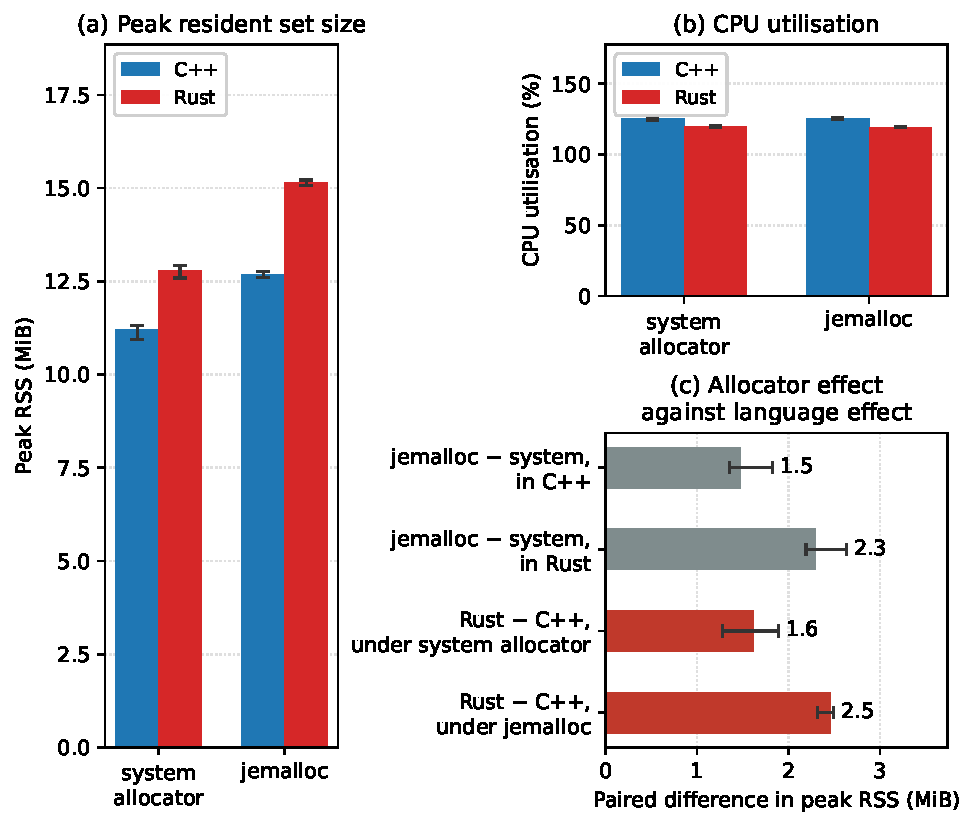
\includegraphics[width=\linewidth]{figures/fig_resources_column.pdf}
\caption[Resource use, and the two effects inside peak RSS]{Resource use at
$\ReprLoad$~kops/s, grouped by allocator. Bars are medians over \NRepeats{}
repeats with bootstrap $95\%$ intervals, and CPU in (b) is summed across
threads.\label{fig:resources}}
\end{figure}

% Same drift as the throughput figure: the RAM chart was opening the safety subsection.
\FloatBarrier
\subsection{Safety via fault injection (RQ2)}\label{sec:safetyresults}
Safe code is checked by putting $\FaultClasses$ defects in. Seven come from inside
the zone Rust claims to govern. Seven were chosen because safe Rust is
meant \emph{not} to stop them. Each one of the first seven is a compile
error in Rust. In C++ each is valid code. The
defect shows up only if a test drives it, and no single sanitiser hits them
all. The use-after-move is the case where no sanitiser flags anything. A
moved-from object is still a valid object. Its value is unset. So there
is nothing wrong to detect, and the name is just lost. All seven
boundary cases compile in safe Rust and fail. On two of them the C++
tools are the ones that flag. LeakSanitizer flags the ref cycle that
Rust leaks in silence, because leaks are safe in Rust by
design~\cite{hughes2025gcrust,cui2024rcanary}. UndefinedBehaviorSanitizer flags
the overflow that Rust defines to wrap. ThreadSanitizer catches the lock-order
inversion in $\DeadlockTsanHits$ of $\DeadlockTsanRuns$ runs, a rate that
itself jumps. It logs lock orders only from locks that work. If the
first inversion waits and never returns, the cycle is never closed, so the tool never
flags it.

The seam double-free is the in-guarantee double-free recast through
\texttt{unsafe}, not a new class. Its C++ half is the same, so only the Rust
column moves. Two Rust model checkers do flag both original boundary defects.
Loom explores thread orders in a sound way. Shuttle picks the ones
Loom cannot reach~\cite{bornholt2021shardstore}. Each had to be written using
the checker's own parts first, and shrunk to model size. Miri flags the
seam double-free, but it reads Rust and cannot run the C++ host the
defect sits behind. LeakSanitizer and UndefinedBehaviorSanitizer flag without
a rewrite. The two model checkers flag the concurrency boundary cases only
after the defect is recast into their parts. Figure~\ref{fig:taxonomy} draws the
whole list as an outcome matrix. Resource Acquisition Is Initialization
(RAII) ties cleanup to object lifetime. It removes the plain missed-unlock,
because leaving a scope destroys the guard and releases its lock. It does not
remove the class: both
forgotten-guard programs hang, and no side's tools said so.

% Full column width no longer fits in the leftover under the safety paragraph.
% [ht] would park the matrix above the next subsection.
\enlargethispage{48pt}
\begin{figure}[!ht]
\centering
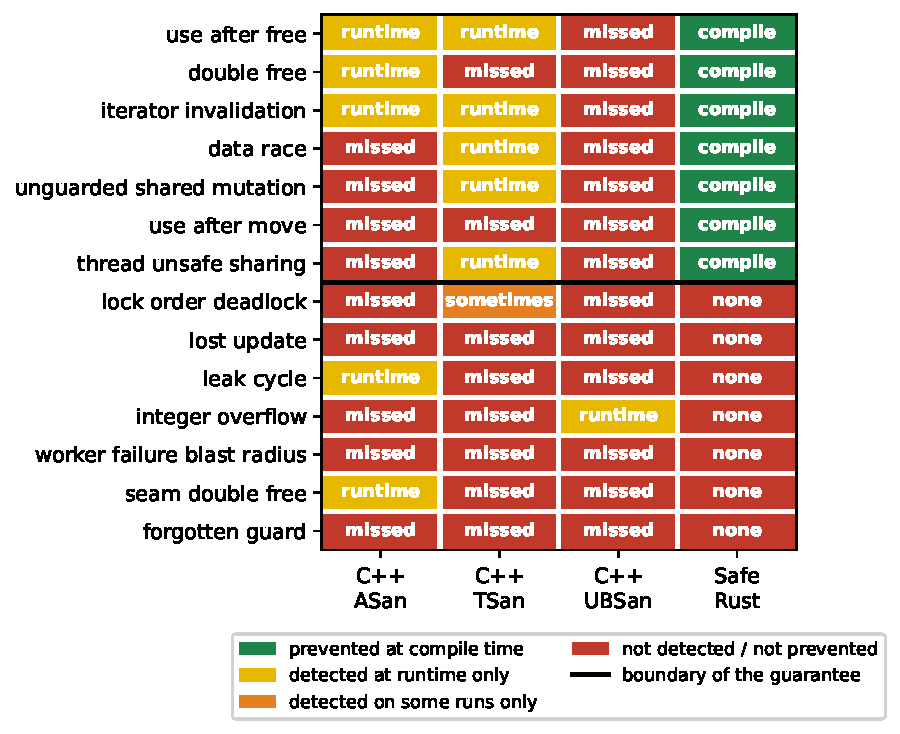
\includegraphics[width=\linewidth]{figures/fig_taxonomy.pdf}
\caption[Where the guarantee stops: the outcome matrix]{The fault-injection
outcomes as a matrix, generated from the taxonomy log.\label{fig:taxonomy}}
\end{figure}

% The outcome matrix was opening the migration subsection. The seam diagram
% does not fit under that matrix, and the following chapter would otherwise
% leave it alone on the next page. The subsection starts on a fresh page so
% the diagram stays with the paragraph that cites it.
\FloatBarrier
\newpage
\subsection{Migration (RQ4)}\label{sec:migrationresults}
The FFI seam, the C-ABI layer between the C++ host and Rust core, is small on
each measured axis: $\FfiEntryPoints$ C entry points in $\FfiSeamLines$ lines
of Rust. All raw-pointer work is kept in
$\FfiUnsafeFns$ functions. The core is left free of \texttt{unsafe}. No extra
cost is seen against the same signal call made directly. That bounds any
per-call tax at $\FfiOpBoundPct\%$ of that call, and
Figure~\ref{fig:ffiseam} shows the structure that bound belongs to. Three
adoption costs beyond the seam were measured as well, and two of them
go against the usual worry about taking Rust.
$\BuildDepShareCpu\%$ of the Rust clean build is third-party code. The project's
own source builds in $\BuildAllFirstPartyCpuRatio$ times the CPU \texttt{g++}
needs. The $\FootShippedRatio\times$ size gap is a linkage policy that
flips when the policy is held fixed. The compared part has no
third-party crates and no \texttt{unsafe} sites ($\DepsCore$ crates,
$\CoreUnsafe$ \texttt{unsafe} sites).

% After the paragraph the leftover is short of the diagram plus caption, so
% [ht] defers it and \chapter flushes it onto an empty float page. A page
% enlarge plus [!ht] keeps the figure with the subsection that cites it.
\enlargethispage{52pt}
\begin{figure}[!ht]
\centering
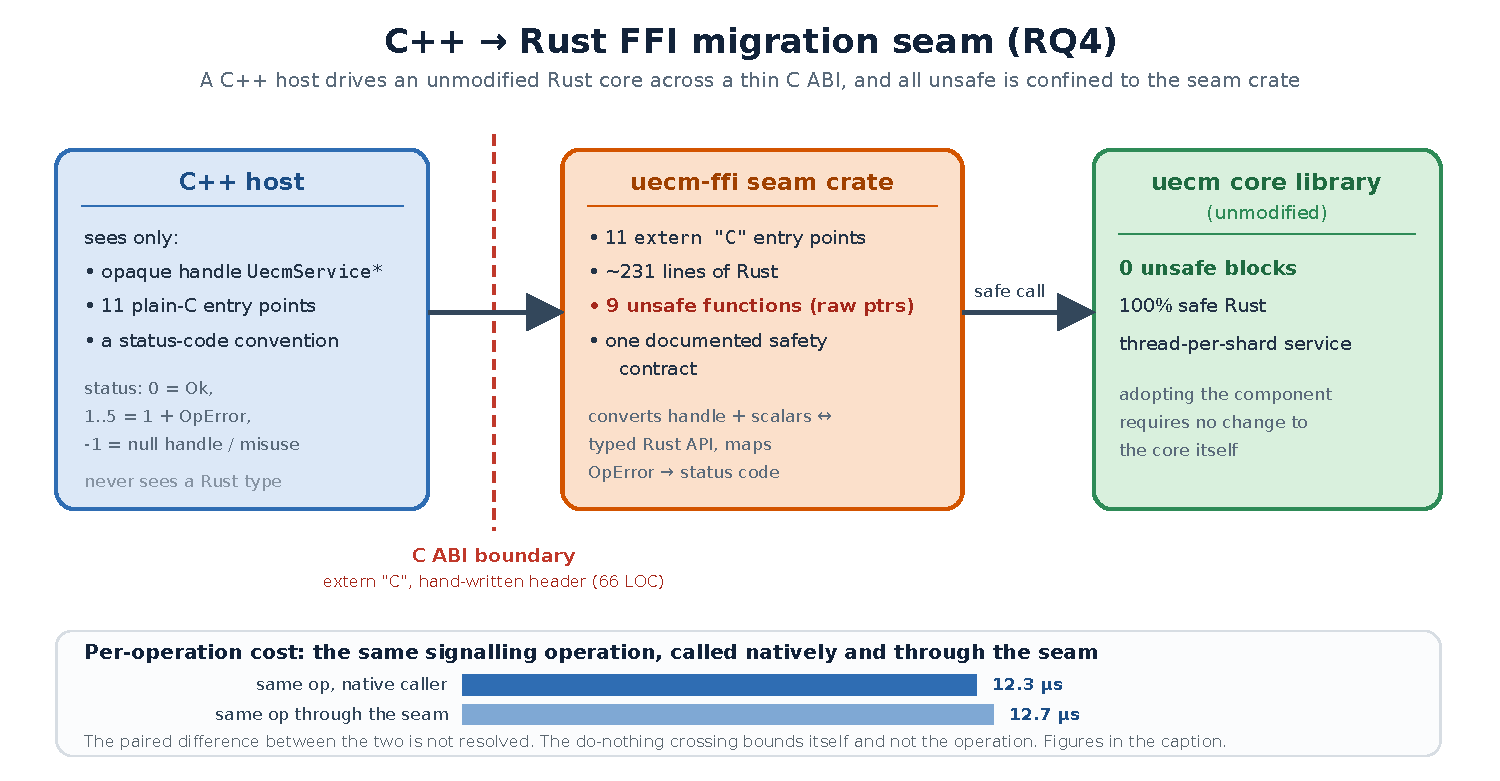
\includegraphics[width=\linewidth]{diagrams/pdf/07_ffi_seam.pdf}
\caption[The C++-to-Rust FFI migration seam]{The C++-to-Rust FFI migration seam.
The same signalling operation costs $\FfiOpNative$~\textmu s directly and
$\FfiOpSeam$~\textmu s through the seam, a paired difference bounded at
$\FfiOpBoundPct\%$ of that call. A do-nothing crossing costs
$\FfiCrossing$~ns and bounds only itself.\label{fig:ffiseam}}
\end{figure}

\chapter{Discussion\label{chapter:discussion}}

\section{Summary of findings}
At $\ReprLoad$~kops/s the variants agree to
$\PFiftyRange\,\mu$s at the median, and the pooled far tail lands on
\FarTailLower{}'s side. The end-to-end round-trip is only
$\BudgetCoreShareMax\%$ language work, so it cannot bound a language effect.
The same core timed apart is $\BudgetCoreRatio\times$ faster in
\BudgetCoreFaster{}. At higher loads the campaign clock shows an allocator
split at $\KneeSplitLoad$~kops/s and a $\OverloadThrRatio\times$ lead for
\OverloadSustainedFaster{} at $\OverloadLoad$. Moving the fill after the
window on this same host removes both large patterns and leaves a smaller
Rust lead. CPU per completed call falls from $\OverloadCpuPerOpRatio\times$
to $\ProbeAfterCpuPerOpRatio\times$. Neither overload clock supplies
service-latency percentiles, so RQ1 has no language verdict after saturation. The RQ2 outcome
is complete for the fourteen-class catalogue set in advance and does not
depend on the host. All seven in-guarantee classes are
compile errors in safe Rust. All seven boundary classes compile and
fail in Rust and in C++. RQ3 finds a higher Rust peak RSS under both heaps:
$\RssLangDiffLo$--$\RssLangDiffHi$~MiB on the campaign host,
$\GuestRssLangLo$--$\GuestRssLangHi$ on the guest, and
$\BmRssLangLo$--$\BmRssLangHi$ on the second bare-metal host. Below
saturation Rust draws slightly less CPU. Corrected high-load throughput gives
no general language rank. RQ4 finds a small seam whose per-call tax is bounded
at $\FfiOpBoundPct\%$ of that call. API design and learning remain
literature-backed adoption costs that this study does not measure directly.

\section{Discussion on the research questions}\label{sec:rqdiscussion}
RQ1 has two answers separated by regime. At $\ReprLoad$~kops/s the campaign
resolves median, p99 and p99.9 differences, and the pooled p99.99 lies on
Rust's side. The end-to-end clock still cannot bound a language effect because
the core call is only $\BudgetCoreShareMax\%$ of what it times. After
saturation neither available percentile clock estimates service latency. The
campaign includes producer-side fill, while Clock B measures cumulative
schedule drift. No overload tail ranking follows.

The campaign throughput shows an allocator split at one rung and a C++ lead
later. Clock B, on this same host, removes both large patterns when the fill
is deferred and leaves a smaller Rust lead. That isolates the fill as the
source of the large gaps. The smaller lead is reported and not explained.
This visit took no allocation profile, and the queue and channel
substitutions belong to an earlier host. Clock A's
lower Rust p99 is deliberately coordinated-omission biased and is not an RQ1
tail result. Clock B's throughput is a completed-work comparison. Its
percentiles are schedule drift. The closest prior work reports
similar degradation past a threshold rate and attributes it to stackless
\texttt{async}/\texttt{await}~\cite{arvidsson2025async}. That cause cannot
carry here because neither side uses an asynchronous runtime. Changing Rust's
reply handle, on an earlier host, does not explain the smaller lead that
remains here. The campaign ratio therefore
remains a result for its harness and does not rank top service rates. The
prediction logged in advance had instead named bounds and overflow
checking~\cite{zhang2022runtime,harris2023morello}. That part was wrong. At
nominal load the median result still fits evidence that Rust's safe checks are
mostly absorbed by modern out-of-order
CPUs~\cite{balasubramanian2017rust,emmerich2019drivers}.

On safe code some defects are compile errors, so they never become a program that can run. The seven classes Rust
does not stop are part of the answer, not a warning added then. A
compiler that will not build a program rules the defect out of each
run. A sanitiser rules it out only of the
runs a sanitiser test happens to take. What is fixed there is the
run coverage, not the breadth of the list.
Figure~\ref{fig:boundary} names the way on each side of that line. Rust
reasons about aliasing and not about lock order. A \texttt{Mutex} guard
whose life the borrow checker tracks well says nothing about whether
two threads take their locks in a matching
order. Static deadlock checks for Rust are an open research
problem~\cite{zhang2026deadlock}. The lost update misses ThreadSanitizer for the
same reason it misses the borrow checker. Where each access is synced
right, there is no unsynced access to find. In a field study of
$105$ real concurrency bugs, about a third of the cases that were not deadlocks broke
the order the writers meant, not their
locking~\cite{lu2008mistakes}. Taking Rust drops one class of concurrency
defect and leaves in place the class that fails in silence. A plan to move that
reads ``memory-safe'' as ``concurrency-safe'' would mis-budget its review
effort. In the corpus of Xu et al., every published Rust Common
Vulnerabilities and Exposures (CVE) memory-safety entry but one compiler bug
involves \texttt{unsafe}~\cite{xu2021rustcve}.
That is why keeping the core free of \texttt{unsafe} matters. It is also why unsafe
spreading through crates is a review concern~\cite{evans2020rust}.

\begin{figure}[ht]
\centering
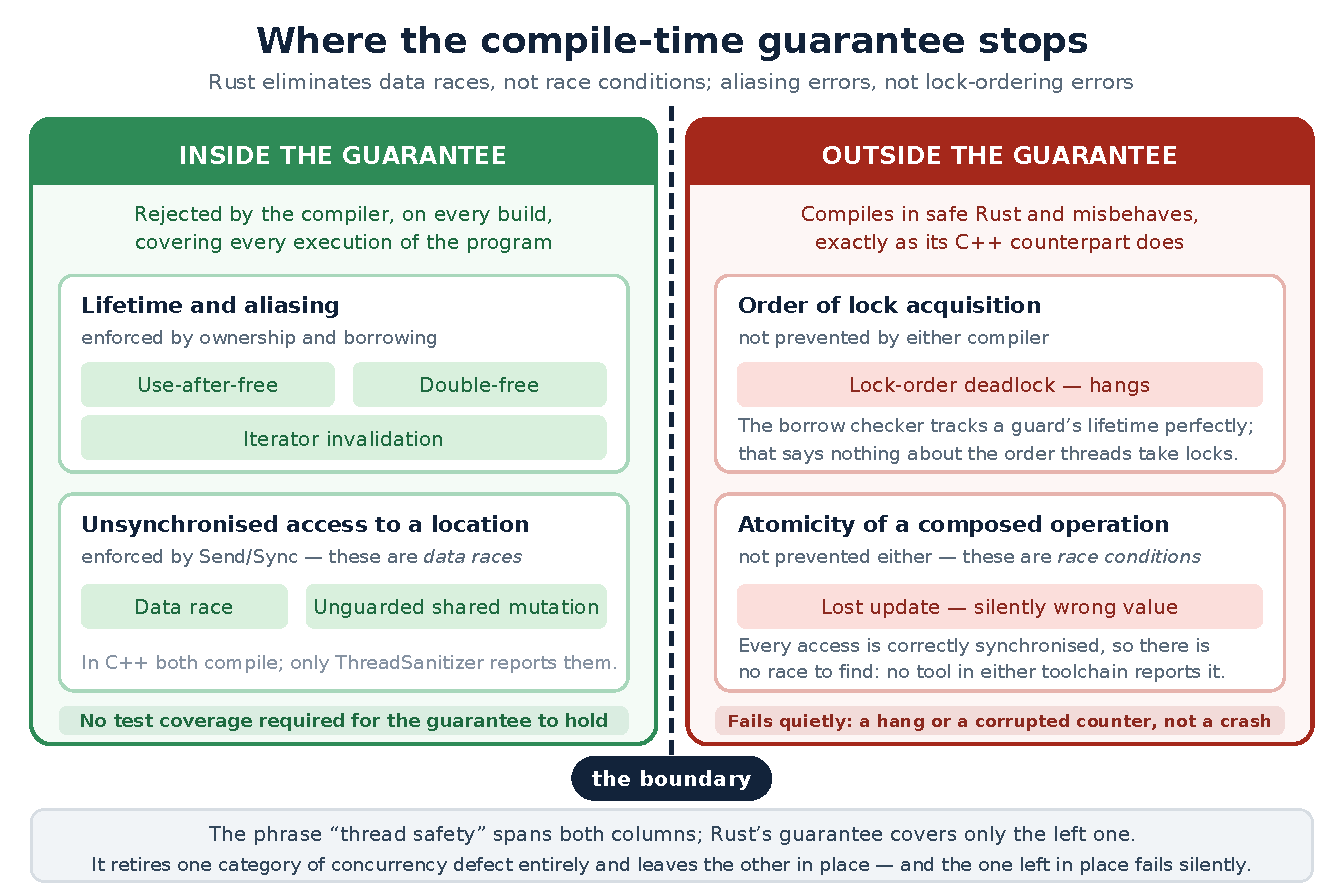
\includegraphics[width=0.78\linewidth]{diagrams/pdf/17_guarantee_boundary.pdf}
\caption[Where Rust's compile-time guarantee stops]{Where Rust's compile-time
guarantee stops, with classes grouped by the mechanism that rejects
them.\label{fig:boundary}}
\end{figure}

One case reaches past the fault programs. A spec gap let a
call be sent outside the service running window. It passed each
test, each parity vector and all three sanitisers because nothing ever called
that path. What turned undefined behaviour into a catchable failure on the
Rust side was a plain bounds check, not a proof. The thing worth
planning for is ``checked by default'', not ``ruled out at compile time''. The
root cause belongs to the method. A ban stated without a way
behind it leaves each version to fail in its own idiom.

RQ3 splits by resource and the splits do not point the same way. The RAM
cost holds under both heaps and on a second host with a
new compiler. Peak RSS is a max for the whole run, so the jitter that
destroys a p99 does not touch it. Sized against the heap's own effect, the
two are of the same order on both bare-metal hosts. On the guest the
heap's was an order of magnitude larger. The language effect travels. The
ratio does not. The quiet host also puts the cost past the heap, by
the heap's own counts. One close study reports the other sign, with
Rust lowest and the gap growing as concurrency rises~\cite{karlback2021ran}.
Those two findings agree once the variants are read as two concurrency runtimes, not two sides.
Their C++ runs on Boost.Fibers, which gets a stack per fiber. Their Rust
runs on Tokio, where a task is a small future on the heap. What they
timed is the per-task cost of two concurrency runtimes.
Two further studies agree with the way found
here~\cite{olsson2023ranmgmt,sundvisson2026drivers}. Below saturation Rust
draws slightly less CPU. The larger flip under the campaign clock is the
recorder. On this host it is absent once the fill moves, and it cannot be
assigned to Rust's safe code model. A smaller throughput lead remains.

RQ4 finds a small machine-side seam. A C++ host can
call an unchanged Rust core across a thin C-ABI seam whose cost on a real
signal call is bounded at $\FfiOpBoundPct\%$ of that call. Prior work identifies
design and learning as human costs~\cite{fulton2021adopting,crichton2024learning},
but this study does not measure their size. Keeping \texttt{unsafe}
at the seam bounds what has to be checked, not what can be corrupted. Host and
part share one address
space~\cite{rivera2021galeed,kirth2022pkrusafe}. The build and footprint axes
point the same way as the seam. A vendor worried about either should
audit its crate budget before blaming the compiler. The one axis where C++
leads outright is the edit and compile loop for changes that stay inside one
source file. The $\FootShippedRatio\times$ size figure sets two
linkage policies, and the order flips when the policy is held fixed.

\section{Revisiting the hypotheses}\label{sec:hypotheses}
Section~\ref{sec:rqs} set three hypotheses before any run.
Saying how they came out is what sets a test apart from a sketch.

\begin{description}
  \item[H1] It is not accepted as written. No equivalence margin was defined,
        so a small significant median difference cannot establish
        performance equivalence. At $\ReprLoad$~kops/s the paired test resolves
        $\PFiftyDiffAbsMax\,\mu$s and higher-percentile differences, while the
        pooled far tail favours Rust. The isolated core favours
        \BudgetCoreFaster{}. After saturation the available clocks do not
        provide a valid service-latency ranking. The hypothesis combined the
        round-trip, core code, recorder work and overload behaviour into one
        quantity that the method cannot support.
  \item[H2] For the seven injected classes of its kind it holds without
        exception. It fails in the looser reading its wording invites. It is
        accepted for memory safety and data-race freedom, rejected for
        concurrency correctness at large, and it is a claim about \emph{safe}
        Rust only. The seam case shows the same class returning inside
        \texttt{unsafe}.
  \item[H3] Any per-call tax is bounded at $\FfiOpBoundPct\%$ of that signalling call. This is
        supported by the upper bound on the paired difference. A non-significant
        difference alone would not show that the tax is small. The accompanying claim, that the real
        cost is design and training, is supported structurally and not
        statistically.
\end{description}

\section{Engineering guidelines for incremental adoption}\label{sec:guidelines}
The rules are the practical form of the findings, and each carries the
limit of the finding behind it. Choose a first part for how thin its API is,
not for its size. The rewrite of a rich interface is the
schedule risk. The edge itself is not. Keep the C ABI in its own crate and
the core free of \texttt{unsafe}. That keeps unsafe out of the crate
chains it spreads through~\cite{evans2020rust}. Leave the
concurrency review budget where it is. Prefer a shared-nothing structure in
either language. The strongest concurrency result here belongs to the design and
to neither compiler. Plan the learning curve as a training cost and track
it. Time the part as well as the round-trip. Sweep past the point where
the campaign stops keeping up. Audit every operation on the producer's timed
path, including histogram correction. On this host, running that work after
the timed window removes the large high-load gaps and leaves a smaller
throughput lead.

\section[Where this study sits]{Where this study sits, and what it cannot support}\label{sec:standing}
The studies closest to this one are the five vendor-hosted theses of
Section~\ref{sec:gap}. Their verdicts clash with each other in each way.
The one with the other sign on peak RAM fits this study
once its variants are read as two concurrency runtimes, not two sides.
Four threats still matter, and the first is that one author wrote both
versions. The same failure mode flipped a printed verdict in this
field: comparable after a code review and then Rust worse by $85$--$91\%$
after more speed work~\cite{emberg2023asn1}. The parity suite bounds
what the code does and not speed. The second is that the end-to-end clock
times the design faithfully and the language hardly at all. Third, the
same-host control isolates fill timing. It removes the large campaign gaps
and leaves a smaller Rust lead on the deferred plateau. No allocation profile
was taken on this visit, so that lead is reported and not explained. Clock A
was not repeated here. Fourth, neither high-load clock gives
service-latency percentiles. The campaign includes recorder work, Clock A has
coordinated-omission bias, and Clock B reports schedule drift. The thesis
therefore leaves overload service latency unresolved.

\section{Ethical and professional reflection}
The study uses no personal data, no subscriber data, and no operator secrets. All
traffic is made for the test. The service is based on live code, not
copied from it, so the artefacts can be shared in public. The first
duty is not to claim too much. A vendor could read the RQ2 result as
licence to describe a moved part as ``safe'', and the boundary cases are
why that reading would be wrong. A deadlocked control plane is an outage. A
lost counter update that stays silent can misinform a mobility decision. Nothing
shown here stops either. The second duty is how far the data reaches.
Tail latency numbers from any single host are a thinner
basis for a production roll-out than they look. That is why the earlier
guest sweep is kept, not dropped.

\chapter{Conclusion and Future Work\label{chapter:conclusions}}

The thesis set modern C++ against Rust. The object is a UE Context Management
service. It keeps per-device state, as a gNB-CU-CP does. It looked at four things. Two of them are
how late the tail is, and which defects a compile step can stop. The other two are the
cost of the safe code model and the cost of adding Rust a piece at a time. Both
sides were built against one frozen spec. They were driven along the same code
paths. That is what lets a language effect be told apart from a gap of design or
of skill.

The safety mechanisms act at different stages. Safe Rust rejects all seven
injected memory-safety and data-race classes before they become programs that
can run. The same seven compile in C++, where a sanitiser can report a defect
only if a test executes the relevant path. All seven boundary classes compile
and fail in both languages. On two of them the C++ tools flag what Rust's do
not. Rust therefore drops data races and aliasing errors. It does not drop
race conditions, lock-order errors, leaks, wrapping arithmetic, or the blast
radius of a failed worker. It drops nothing inside an \texttt{unsafe} block.
LeakSanitizer and UndefinedBehaviorSanitizer flag two boundary defects without
a rewrite. The two model checkers flag the concurrency cases only after each
defect is recast into their parts.

On migration the measured machine-side seam is small. An unchanged Rust core
can be driven from C++ across an FFI
seam, the C-ABI layer where the two languages meet. It has
$\FfiEntryPoints$ entry points in $\FfiSeamLines$ lines, and its
$\FfiUnsafeFns$ raw-pointer functions contain all of the \texttt{unsafe}. The
core has $\CoreUnsafe$ \texttt{unsafe} sites. The cost on a real signal call is
bounded at $\FfiOpBoundPct\%$ of that call.
Prior work identifies API design and the learning curve as adoption costs, but
this study does not measure their size.
Most of the Rust build's extra cost is building crates, not the
compiler's own work. The size gap is a linkage policy. The order
rests on which matched policy is chosen. Where C++ leads is the edit and compile
loop. It leads only for edits that stay inside one source file.

On speed the data first splits by what is being timed. The end-to-end clock
starts before a producer sends a request and stops after the worker replies.
It includes the queue, wake-up, and core call. Only
$\BudgetCoreShareMax\%$ of that round-trip is the core work the languages
perform, so this clock cannot bound a compiler effect. A second measurement
removes the queue and cross-thread handoff and times the core call alone. The
core is $\BudgetCoreRatio\times$ faster in \BudgetCoreFaster{} in that
measurement. At the chosen load of $\ReprLoad$~kops/s the paired test finds
$\PFiftyDiffAbsMax\,\mu$s in Rust's favour. At p99.99 the slowest Rust variant sits
$\FarTailLangSep\,\mu$s below the fastest C++ one. The campaign then shows
an allocator split at $\KneeSplitLoad$~kops/s and a $\OverloadThrRatio\times$
C++ lead deeper into overload. Moving the fill after the timed window on
this same host removes both large patterns and leaves a smaller Rust lead.
CPU per completed call falls from $\OverloadCpuPerOpRatio\times$ to
$\ProbeAfterCpuPerOpRatio\times$. The gaps do not rank the two services,
and overload service latency remains unresolved. On RAM
the Rust build carries a few MiB more fixed footprint under both heaps. It does so in
the same direction and MiB scale on all three hosts timed. The
heap choice costs about as much on both bare-metal hosts, and an order of
magnitude more on the guest this study used first.

Taken as a set these support a narrow claim. It is for stateful, concurrent,
partitionable control plane services of this kind. At the loads where the
service still meets its sent rate, the choice is which classes of defect a
team wants to make impossible to write. The other half is whether it will pay the
design and training cost of getting them. Past that point the campaign
includes substantial recorder work and adds no second language rank. What the thesis adds
is not a verdict. It is the frozen spec,
the parity tested pair, and a timing harness that reaches past the saturation
region. A split of the
round-trip says how much of what it times the language can own. A defect
list maps where the guarantee stops.

Future work answers the gaps one at a time. The same-host control is now
done. In-run and deferred fill were repeated on one host, with the pin and
\texttt{nohz\_full} held. The large gaps move with the fill. What remains is
the smaller Rust throughput lead on the deferred plateau, which this visit
does not explain. The next job needs no new host. It is to vary the transparent hugepage policy on one host with all
else held fixed. All three hosts agree that the Rust build carries the larger
footprint. They disagree about how that sits against the cost of the
heap. The guest put it an order of magnitude higher, and neither
bare-metal host does. The hugepage policy is the candidate this study
can name but not test, because it was not the same on each host and only the
system allocator variant gets it. Beyond that, replaying anonymised production
traces would check the call mix. The harness can also take further
control plane parts or the data heavy layer-2 and physical layer (PHY)
path. A part with truly shared mutable state would work the two
sides in a way a shared-nothing design does not. Testing Rust async runtimes against the thread per shard model
would split the runtime from the language in the tail
result~\cite{arvidsson2025async}. Timing what a split of the two
heaps in one process costs would price what keeping a core free of \texttt{unsafe} is
worth~\cite{rivera2021galeed,kirth2022pkrusafe}. A longer case study would track
defect counts and review effort while adding Rust a piece at a time. That is what would
settle the human cost this study can only name.

% Declaration of generative-AI use, required by the University when a language model has
% been used. Shared with Ha_Vien_Mastersthesis_2026.tex: edit ai_statement.tex, not a copy.
%% Declaration of generative-AI use. The University of Helsinki requires a student who
%% has used a language model in preparing a thesis to state in writing which model was
%% used and in what way; the model may not be named as an author or cited as a source.
%%
%% Shared verbatim by Thesis_POC.tex and Thesis_v1.tex so the two cannot drift apart.
%% It uses no generated macros and no chapter numbers, because the two documents number
%% their chapters differently.
%%
%% The order of the paragraphs follows the University's basic reporting instruction:
%% what the use covered, what it was for, which tool, how it performed and how its
%% output was checked, and what the author took from it.

\cleardoublepage
\phantomsection
\addcontentsline{toc}{chapter}{Statement on the Use of AI Tools}
\chapter*{Statement on the Use of AI Tools}
\markboth{Statement on the Use of AI Tools}{Statement on the Use of AI Tools}

\noindent\textbf{Tool.} Anthropic's Claude Opus~5, used through the Cursor development
environment, is the only generative AI system used in the preparation of this thesis. It was
used throughout the work, from June to August~2026. Following University of Helsinki policy the
model is neither named as an author nor cited as a source: it cannot take responsibility for
what it produces, and it cannot reliably vouch for the literature it paraphrases.

\noindent\textbf{What the assistance covered.} It was extensive, and is declared as such. The
model drafted and revised the running prose of this thesis and proposed the order in which its
arguments are made. It wrote and refactored the two implementations of the UE Context
Management service, the load generator, the fault-injection catalogue, and the interoperability
prototype. It wrote the analysis code behind the bootstrap confidence intervals, the exact
paired permutation tests, and the Holm correction, together with the figure-generating and
build scripts and the \LaTeX{} sources. It also suggested candidate literature.
% ==================== ACTION REQUIRED BEFORE SUBMISSION ==========================
% The abstract of Thesis_POC.tex was drafted with model assistance. The University's
% thesis guide states that a language model may not be used when preparing the thesis
% summary, and in this programme the summary also serves as the maturity test, where
% AI use is never permitted. Rewrite the abstract unaided before submitting; until
% that is done the closing sentence of this paragraph is not yet true of Thesis_POC.
% =================================================================================
The abstract was written by the author unaided, as the University's thesis guide requires of
the thesis summary.

\noindent\textbf{What the model did not settle.} The research problem, the four research
questions, and the three hypotheses are the author's, as is the control on which the study's
value rests: freezing one language-neutral specification and one concurrency model, so that the
language remains the only systematic difference between the two implementations. So is the
decision that keeps RQ2 falsifiable, namely to carry two defect classes -- a lock-order deadlock
and a lost update -- that lie outside Rust's compile-time guarantee and can therefore embarrass
the premise rather than confirm it. Every measurement reported here was run by the author on the
hosts documented in this thesis; no measured value came from a language model. Each measured
number reaches the text through a macro regenerated from the raw logs, so a figure cannot be
transcribed by hand, by the author or by the model. The readings of those numbers are the
author's as well, including the two restraints the evidence imposes: that a far tail a
virtualised host cannot resolve must not be reported as equivalence, and that a sweep dominated
by cross-thread handoff cannot bound an effect of the language.

\noindent\textbf{How the output was checked.} Model output was treated as a draft to be
falsified rather than as a result. Claims were checked against the sources cited for them: every
bibliography entry was resolved against Crossref, DataCite, or the issuing body, and each was
traced to the page or clause carrying the claim made of it. That audit found four passages where
the prose overstated or misplaced its source, one of them a sentence inside quotation marks that
does not appear in the work it was attributed to; all four were corrected, and the audit is kept
with the artefacts so that the correction remains reviewable. Code was checked by running it:
the two implementations are held to one conformance suite whose transcripts are diffed line by
line, and the fault catalogue fixes the expected outcome of each defect before it is injected,
so that a surprise appears as a discrepancy instead of being explained away afterwards. Nothing
is asserted here on the model's authority.

\noindent\textbf{What the author took from it.} The model is dependable at mechanical work --
transposing an idiom between two languages, restructuring a table, keeping a build honest -- and
undependable in a specific and predictable way: it will supply a plausible citation for a claim,
a plausible cause for a measurement, and a confident sentence where the data supports a hedge.
Its fluency is not evidence. The lasting lesson of the work was accordingly less about either
language than about verification. The effort saved in drafting is spent again, and rightly, in
checking, and the parts of this thesis that are defensible are the parts that were checked
against a source, a specification, or a measurement.

\noindent\textbf{Responsibility.} The author is responsible for the whole of this thesis: its
language, its facts, its code, its measurements, and its conclusions. Where it is wrong, the
error is the author's.


% STEP 5:
% The bibliography style is selected with the biblatex options in the preamble.

\cleardoublepage %fixes the position of bibliography in bookmarks
\phantomsection

\addcontentsline{toc}{chapter}{\bibname} % This lines adds the bibliography to the ToC
\printbibliography

\backmatter
\begin{appendices}

\appendix{Key terms\label{appendix:terms}}
Table~\ref{tab:abbrev} collects the terms used throughout the thesis that are not acronyms, for
readers outside the telecom domain. The acronyms are written out at first use and listed together
in the \nomname{} on page~\pageref{page:acronyms}.

\begin{table}[H]
\centering
\caption[Key terms]{Key terms used throughout the thesis.\label{tab:abbrev}}
\singlespacing
\footnotesize
\renewcommand{\arraystretch}{1.2}
\begin{tabular}{@{}p{0.21\linewidth} p{0.71\linewidth}@{}}
\hline\hline
Term & Meaning \\
\hline
Control plane & The signalling and management path, as opposed to the user-plane data path \\
Tail latency & High-percentile latency (p99, p99.9, p99.99), the worst-case-oriented timing metric \\
Jitter & How much latency varies from one operation to the next, as opposed to its typical value \\
Saturation & The offered load beyond which the service can no longer keep up and requests start queueing \\
Shard & One of several independent slices of the UE state, each owned by exactly one worker thread \\
Open-loop & A load schedule whose send times are fixed in advance, so a slow response delays no later request \\
Coordinated omission & The bias an open-loop schedule avoids, in which a stalled client stops issuing requests and so never records the latency of the stall \\
\hline
\end{tabular}
\end{table}

% In the full draft this is Appendix D. Here it is Appendix B because Thesis_v4
% carries only Key terms before it. The label stays appendix:config so both
% documents share one cross-reference name.
\appendix{Host and campaign configuration\label{appendix:config}}
Table~\ref{tab:testbed} itemises the three machines the campaigns ran on: the bare-metal host of
Section~\ref{sec:testbed} that every performance and resource table of the main sweep is drawn from,
the virtualised host it replaced, and the second bare-metal host at a different design that
Section~\ref{sec:testbed} reads against it. The resident-set decomposition belongs to the
second bare-metal host and is reported in Section~\ref{sec:resources}. The fault catalogue was
compiled and run on the development machine, whose toolchain its own caption records. Of the
adoption-cost axes only build time is host-sensitive, which is why that one is reported as a
paired ratio while the footprint and dependency figures are deterministic. The three small paired
experiments predate the move to bare metal and carry no environment record, so each supports a
ratio between two variants measured alternately in one session. Section~\ref{sec:testbed} points
here for the field-by-field record of what each campaign captured. Every column reports what was
measured, and the protocol they are read against is published as \texttt{bench/TESTBED.md}.
Table~\ref{tab:params} gathers the configuration of the service, the workload and the campaign.

% [tp] and not [H]: measured in the full draft. At [H] the table did not fit under its
% own intro paragraph, and [H] forbids the following text from flowing back into the gap.
\begin{table}[tp]
\centering
\small
\caption[The three measurement hosts]{The three machines the campaigns ran on, each reported as
measured. Every hardware, kernel and toolchain cell is generated from that campaign's own
environment capture rather than restated from the protocol of \texttt{bench/TESTBED.md}. The
operating-system row names the machine and, where a campaign ran in a container, the image's
userland beside it, so the kernel row prints one value for both. The last
two rows are prose, because what an instrument set is adequate for is a judgement and not a captured
field. The columns are arranged so that each
adjacent pair isolates one change, with the exceptions the Kernel and Toolchain rows record.
Reported sweep against virtualised host: the same design and the same container image on a
different machine, one \texttt{g++} release apart within GCC~15, which is what
Section~\ref{sec:testbed} reads a hardware effect from.
Reported sweep against second bare-metal host: a different shard count, load grid, repeat count and
compiler on comparable hardware, which is what tests whether the findings depend on those choices.
Rows where all three agree describe the source or the method rather than any machine. The
\emph{Short of protocol} marks are deliberate and are argued where they appear.\label{tab:testbed}}
\renewcommand{\arraystretch}{1.1}
\footnotesize
\begin{tabular}{@{}R{0.14\linewidth} R{0.26\linewidth} R{0.27\linewidth} R{0.25\linewidth}@{}}
\hline\hline
Aspect & Reported sweep & Virtualised host, same design & Second bare-metal host, different design \\
\hline
Host & \MainCpu{}, \MainCores{} cores, \MainSockets{} socket & \GuestCpu{} guest, \GuestCores{} vCPUs & \BmCpu{}, \BmCores{} cores, \BmSockets{} socket \\
Operating system & \MainHostDistro{}. Image \MainDistro{} & \GuestDistro{} & \BmDistro{} \\
Kernel & \MainKernel{} & \GuestKernel{} & \BmKernel{} \\
Hypervisor & \MainVirt{}. Governor \MainGovernor{}, boost off, verified on the machine & \GuestVirt{}. Frequency and turbo host-controlled, unobservable from inside & \BmVirt{}. Governor \BmGovernor{}, verified on the machine \\
CPU steal & None: no hypervisor to lose a timeslice to & Not characterised. The capture's single one-second sample read \GuestSteal{}, and no steal probe was run on this host & \BmStealWithSteal{} of \BmStealIntervals{} intervals on \BmStealCores{} pinned cores \\
Isolation & \texttt{nohz\_full} \MainNohzFull{}. \texttt{isolcpus} \MainIsolcpus{}, omitted on purpose (\S\ref{sec:testbed}) & \texttt{isolcpus} \GuestIsolcpus{}, \texttt{nohz\_full} \GuestNohzFull{} & \texttt{isolcpus} \BmIsolcpus{}, \texttt{nohz\_full} \BmNohzFull{}. \emph{Short of protocol} \\
Hugepages & \MainThp{} & \GuestThp{}, and only the system-allocator variant inherits it & \BmThp{} \\
Toolchain & \texttt{g++~\MainGpp}, \texttt{rustc~\MainRustc}, pinned in a container image & \texttt{g++~\GuestGpp}, \texttt{rustc~\GuestRustc} & \texttt{g++~\BmGpp}, \texttt{rustc~\BmRustc}, so a compiler change is tested too \\
Pinning & Cores \MainPinned{}, $7$ shards, $7$ producers & Cores $2$--$15$, \GuestShards{} shards, \GuestProducers{} producers & Cores \BmPinned{}, \BmShards{} shards, \BmProducers{} producers \\
SMT & \MainSmt{}, verified & Absent from the topology the guest is shown, and decided on the host & \BmSmt{}, verified \\
Repeats & \NRepeats{} over \NLoadLevels{} loads, \NRuns{} runs & \GuestRepeats{} over \GuestLoadLevels{} loads, \GuestRuns{} runs & \BmRepeats{} over \BmLoadLevels{} loads, \BmRuns{} runs. \emph{Short of protocol} \\
Instruments & Counters, pooled HDR sidecars, jitter, allocator accounting & None available in the guest & Counters at two scopes, HDR sidecars, allocator accounting \\
\hline
Adequate for & The pre-committed campaign-clock results. Not overload service latency & Everything except the far tail below saturation & Confirming campaign-clock directions survive a change of design \\
\hline
\end{tabular}
\end{table}

\begin{table}[ht]
\centering
\small
\caption[Configuration of the service, the workload, and the campaign]{Configuration of the service under test, the workload driving it, and the measurement
campaign. Service parameters are fixed by the frozen specification, with one exception: the
shard count is set to match the cores the host offers (Section~\ref{sec:testbed}). All of them,
that one included, are identical in both languages. Campaign figures are generated from the
measurement logs together with the
tables that report them. The representative load is fixed rather than derived, for the reason
Section~\ref{sec:workload} gives, and the throughput plateau is the lowest of the four variants'
own plateaus, which differ.\label{tab:params}}
\footnotesize
\renewcommand{\arraystretch}{1.05}
\begin{tabular}{@{}R{0.28\linewidth} R{0.28\linewidth} R{0.36\linewidth}@{}}
\hline\hline
Parameter & Value & Note \\
\hline
\multicolumn{3}{@{}l}{\emph{Service under test, identical in both languages}} \\
Shards, and worker threads & $7$ & one thread owns one shard. Identical in both languages, which is what the fairness control requires (\S\ref{sec:controlsbrief}) \\
Queue bound per shard & $1\,024$ requests & bounded and blocking, so overload is observable \\
Initial map capacity & $4\,096$ entries & reserved so steady state does not rehash \\
Bearers per context & at most $8$ & \\
Signaling payload & $64$ bytes & \\
Context ceiling per shard & $200\,000$ & \\
Shard selection & SplitMix64, then modulo & pinned: diffuses sequential identifiers \\
Intra-shard hash & FNV-1a, 64-bit & pinned on both sides and checked bit-for-bit \\
\hline
\multicolumn{3}{@{}l}{\emph{Workload}} \\
Workloads & signal, mixed & mixed walks the full RAN lifecycle \\
Active UEs & \SweepUes{} & \\
Offered-load levels & \NLoadLevels{} & up to $\MaxOfferedLoad$~kops/s \\
Representative load & $\ReprLoad$~kops/s & fixed, see caption \\
Campaign-clock throughput plateau & $\SatKnee$~kops/s achieved & both languages track through $\TrackingLoad$~kops/s. At $\KneeSplitLoad$ the Rust heaps split, and deferred fill on this host removes that split (Section~\ref{sec:overload}) \\
Load model & open loop, fixed intended schedule & latency measured from intended send time \\
\hline
\multicolumn{3}{@{}l}{\emph{Campaign}} \\
Build variants & $\NVariants$ & two languages $\times$ two allocators \\
Repeats per sweep point & \NRepeats{} & variants interleaved within each repeat \\
Measured runs & $\NRuns$ & \\
Latency capture & HDR histogram, $[1\,\text{ns}, 3.6\,\text{s}]$, 3 s.f. & same algorithm and configuration on both sides \\
Summary statistic & median with bootstrap $95\%$ confidence interval & intervals reported in full, not as half-widths \\
Language comparison & exact paired permutation test & \NTests{} tests, Holm-corrected \\
Attainable $p$ floors & $\MinAttainableP$ / $\CorrectedFloor$ & uncorrected / after correction \\
\hline
\end{tabular}
\end{table}

\paragraph{What each campaign recorded.}
Each of the $\NRuns$ runs of the factorial design in Table~\ref{tab:params} contributes one
newline-delimited JSON record. Nothing is aggregated at capture time. A record carries the
configuration (language, allocator, workload, shard and producer counts, target rate), the
outcome (operations completed, errors, wall-clock duration, achieved throughput), the latency
distribution from the HDR histogram (mean, standard deviation, the quartiles, p50, p90, p99,
p99.9, p99.99 and the maximum, in nanoseconds), a shorter block for inter-operation latency
variation (mean, standard deviation, p50, p99, p99.9, the maximum and a sample count), the
resource counters from \texttt{getrusage} (peak resident set size, user and system CPU seconds,
CPU utilisation), and the per-operation-kind counts. A \texttt{jemalloc} variant adds that
allocator's own accounting. A system-allocator variant stores those fields as unavailable rather than
as zero, on the same principle as the governor and turbo state. The kind counts are what makes a
divergence between the languages show up as a parity failure (Chapter~\ref{chapter:design}) instead
of a performance difference. Each run also persists its complete HDR bucket contents to a sidecar,
so the repeats can be pooled before a far-tail percentile is read
(Section~\ref{sec:statsbrief}), and a separate file records \texttt{perf} counters at two scopes, the
end-to-end path and the operation on its own.

The three small paired experiments have a different shape. For each of \BudgetRepeats{}
interleaved repeats the decomposition records the batch-mean cost in both languages, once for
the operation called directly and once through the threaded service. A third dataset of the same
shape over \ContentionRepeats{} repeats records sustained throughput through the bounded queue and
completion primitives alone. The FFI comparison of
Section~\ref{sec:migrationresults} has that structure over \FfiOpRepeats{} repeats. All three
predate the environment record, which is why each is read as a ratio between its two variants.

Build time is the one RQ4 axis that is a timing measurement. It is recorded over
\AdoptRepeats{} interleaved repeats at \AdoptJobs{} parallel jobs on the development machine,
alternating the toolchains so the ratio survives a change of machine even though the seconds do
not. The static footprint and the resolved dependency graph are read from the linked binaries
and the manifests.

The fault catalogue is categorical. Each of the $\FaultClasses$ cases yields four tool logs
(AddressSanitizer, ThreadSanitizer and UndefinedBehaviorSanitizer on the C++ program, and
\texttt{rustc} on the safe-Rust counterpart) and one taxonomy row carrying the three sanitiser
outcomes, the detection stage, the compiler result, and the expectation registered before the
study. The two original boundary cases yield a second table from the model checkers, and the
\texttt{unsafe} one a third from the interpreter. The table and figure in
Section~\ref{sec:safetyresults} are generated from those logs.

Every load sweep writes the environment record of Section~\ref{sec:repro} beside its results,
including the fields a given host does not expose. The governor and turbo state are stored as
unavailable rather than left out, so the limitation of Section~\ref{sec:testbed} is a property
of the dataset. The virtualised campaign shares the sweep's design and predates the later
instruments: its records carry the percentiles and the resource counters and nothing else. That
absence is the measurement-validity argument of Section~\ref{sec:testbed}, which is why the
campaign is kept. The second bare-metal campaign carries the same record shape as the reported
sweep, including the allocator accounting that lets Section~\ref{sec:resources} decompose the
resident set, but runs a different shard count, load grid, repeat count and toolchain. Each
campaign has its own generator and macro prefix.

The two clock diagnostics each cover the same fourteen-load, two-language,
two-allocator grid. Clock B is this host. The processor is \ProbeAfterCpu{},
the pin is \ProbeAfterPinned{}, and \texttt{nohz\_full} is
\ProbeAfterNohzFull{}, matching the campaign's \MainCpu{} and
\texttt{\MainNohzFull}. Clock A was not repeated here and remains an earlier
host, so it cannot supply this campaign's percentiles. Clock B defers the
fill, and its overload percentiles are schedule drift. At the top load Rust
is ahead on both heaps, at $p \ProbeAfterThrPSystem$ on the system allocator
and $p \ProbeAfterThrPJemalloc$ under \texttt{jemalloc}. CPU per completed
operation is $\ProbeAfterCpuPerOpRatio$, against $\OverloadCpuPerOpRatio$
while the fill ran inside the window. The large ratio is the recorder. The
smaller throughput lead remains.

The tables that follow are the measurements the main text cites from this appendix.

\begin{table}[ht]
\centering
\small
\caption[Inter-operation jitter at the representative load]{Inter-operation latency variation at a
sustained offered load of $\ReprLoad$~kops/s, in microseconds, as a median over \NRepeats{}
interleaved repeats with a bootstrap $95\%$ interval. Measured within one producer and never across
producers, since two producers share no schedule and a difference between them is not a variation
either one experienced. Reported for completeness rather than as evidence: no research question
names this metric, and it is absent from the paired family of
Section~\ref{sec:statsbrief}.\label{tab:jitter}}
\begin{tabular}{@{}l r r r r@{}}
\hline\hline
Variant & p50 & p99 & p99.9 & max \\
\hline
C++ (system alloc) & \mci{1.5}{1.3}{1.6} & \mci{19.4}{13.9}{23.1} & \mci{44.3}{42.7}{47.3} & \mci{169.9}{165.8}{202.9} \\
C++ (jemalloc) & \mci{1.5}{1.4}{1.6} & \mci{23.4}{18.1}{31.3} & \mci{44.0}{41.7}{46.0} & \mci{173.8}{154.9}{185.9} \\
Rust (system alloc) & \mci{1.4}{1.2}{1.5} & \mci{25.1}{17.8}{31.7} & \mci{45.1}{42.4}{46.6} & \mci{106.7}{60.7}{113.0} \\
Rust (jemalloc) & \mci{1.7}{1.6}{1.8} & \mci{25.4}{19.7}{29.7} & \mci{43.8}{41.1}{46.2} & \mci{74.7}{57.8}{115.3}
\\
\hline
\end{tabular}
\end{table}

\begin{table}[ht]
\centering
\small
\caption[The resident set decomposed by the allocator]{Where the peak resident set goes on the
second bare-metal host, from \texttt{jemalloc}'s own accounting in each of the \BmJeRuns{} runs of
the two \texttt{jemalloc} variants. Medians in MiB over the steady-state loads, with the paired language
difference in the last column. The two rows below the rule are the argument: the allocator holds
\emph{less} in the Rust build, and the process holds more, so the difference is outside the
allocator. The final row is the quantity the other rows decompose. The derived row is the median of
the per-run difference and not the difference of two medians, because the two figures it subtracts
come from one process at one moment, so the column does not sum
exactly.\label{tab:resident}}
\begin{tabular}{@{}l r r r@{}}
\hline\hline
Component & C++ & Rust & Difference \\
\hline
Live allocation (\texttt{allocated}) & 0.78 & 0.62 & $-0.16$ \\
In active pages (\texttt{active}) & 1.43 & 0.79 & $-0.64$ \\
Arena bookkeeping (\texttt{metadata}) & 4.19 & 6.26 & $+2.07$ \\
Resident in allocator mappings (\texttt{resident}) & 11.02 & 9.10 & $-1.92$ \\
\hline
Outside those mappings (derived) & 4.04 & 7.86 & $+3.82$ \\
Peak resident set (\texttt{getrusage}) & 15.08 & 16.82 & $+1.74$\\
\hline
\end{tabular}
\end{table}

The allocation profile on the second bare-metal host was taken to name the call sites behind
the resident-set difference of Section~\ref{sec:resources}. Two departures from the campaign
explain why it cannot. The first profile ran closed loop at $\BmProfThroughput$~kops/s, past the
plateau bracketed at $\BmKneeLo$--$\BmKneeHi$~kops/s. Repeating it at a swept load below saturation
shrank the discrepancy by most of its size and did not remove it. What remains is that
profiling requires an allocator built to sample every allocation and record a backtrace, so the
variant under profile is not the variant the campaign measured. Each symbolised profile puts almost all
of its flat bytes on a frame that allocates nothing, $\BmProfFlatCppPct\%$ on a deallocation
symbol in the C++ variant and $\BmProfFlatRustPct\%$ on the allocator's own backtrace routine in the
Rust one. Attributing the footprint would need a profile taken at a swept load, on a build
whose peak RSS reproduces the campaign's ordering.

\end{appendices}

% The class writes the page counts for the abstract form from \AtEndDocument, which
% runs before \end{document} flushes the last page. Without this the final appendix
% page is never counted and the form reports no appendix pages at all.
\clearpage

\end{document}
